\documentclass[11pt,a4paper]{article}
\usepackage[margin=2.2cm]{geometry}
\usepackage[T1]{fontenc}
\usepackage{lmodern}
\usepackage{microtype}
\usepackage{graphicx}
\usepackage{booktabs}
\usepackage{longtable}
\usepackage{array}
\usepackage{tabularx}
\usepackage{xcolor}
\usepackage{enumitem}
\usepackage{listings}
\usepackage[most]{tcolorbox}
\usepackage{amsmath,amssymb}
\usepackage{tikz}
\usetikzlibrary{arrows.meta,positioning,fit,calc}
\usepackage[colorlinks=true,linkcolor=blue!50!black,urlcolor=blue!50!black]{hyperref}
\usepackage{titlesec}
\usepackage{fancyhdr}

\graphicspath{{../figs/}}
\setlist{itemsep=2pt,topsep=3pt}
\setlength{\parskip}{4pt}
\setlength{\parindent}{0pt}
\emergencystretch=3em

\definecolor{codebg}{gray}{0.95}
\lstset{basicstyle=\ttfamily\small,backgroundcolor=\color{codebg},frame=single,framerule=0pt,
        breaklines=true,columns=fullflexible,keepspaces=true,showstringspaces=false,
        literate={≥}{{$\geq$}}1 {≤}{{$\leq$}}1 {→}{{$\rightarrow$}}1}

\newtcolorbox{keybox}[1][]{colback=blue!4,colframe=blue!45!black,fonttitle=\bfseries,title={#1},boxrule=0.6pt,arc=2pt}
\newtcolorbox{warnbox}[1][]{colback=orange!6,colframe=orange!70!black,fonttitle=\bfseries,title={#1},boxrule=0.6pt,arc=2pt}
\newtcolorbox{qbox}{colback=gray!5,colframe=gray!55,boxrule=0.4pt,arc=2pt,left=4pt,right=4pt,top=2pt,bottom=2pt}
\newcommand{\Q}[2]{\begin{qbox}\textbf{Q: #1}\par\smallskip #2\end{qbox}}
\newcommand{\file}[1]{\texttt{\detokenize{#1}}}
\usepackage{xspace}
\newcommand{\pg}{PostgreSQL\xspace}
\makeatletter\newcommand{\rows}[1]{\@@input #1 }\makeatother  % primitive input: works inside longtable

\pagestyle{fancy}
\fancyhf{}
\lhead{\small CS-5187 A3 --- LLM-Guided Grammar-Aware Fuzzing of PostgreSQL}
\rhead{\small Project guide}
\cfoot{\thepage}

\title{\textbf{LLM-Guided Grammar-Aware Fuzzing of PostgreSQL}\\[4pt]
\large The whole project: what we built, what happened, and why\\[2pt]
\normalsize Study guide for progress meeting 2 (CS-5187 Term Project A3)}
\author{Venu, Bhuvan, Gowtham}
\date{Status: 24 October 2026}

\begin{document}
\maketitle
\thispagestyle{empty}

\begin{keybox}[How to use this document]
Read Part~I (one page) and the numbers cheat sheet (Section~\ref{sec:cheat}) first:
together they answer most questions in a meeting. Parts~II--VI explain every
component in depth: what it does, why it is built this way, and what it was
measured to do. Part~VII is a long list of questions the professor may ask,
each with a short answer we can give out loud. Every number in this document
comes from a run recorded in the repository (path given) or is marked
\emph{planned}.
\end{keybox}

\tableofcontents
\clearpage

\part{The project in brief}

\section{The project on one page}
\label{sec:onepage}

\paragraph{The problem.} \pg is the most widely used open-source relational
database. Its query planner and executor change every week on the
development branch (\emph{master}). The most harmful bugs are \emph{wrong
results}: a query returns the wrong rows, without an error, without a crash,
without any trace in the logs. Fuzzers for database systems mostly find
crashes; tools that find wrong results (SQLancer: TLP, NoREC, PQS) use small,
hand-written query generators. Neither line of work knows what changed in the
code yesterday.

\paragraph{Our idea in one sentence.} Generate SQL from a \emph{typed grammar}
and keep every generated query as a \emph{derivation tree}; use that tree for
four jobs (generation, mutation, metamorphic oracles, and reduction of
failures); and let an LLM read recent \pg commits and \emph{extend} the grammar
and the oracle, while a validation gate on a real server decides what the
LLM output is allowed to change.

\paragraph{The experiment (backbone of the paper).} Three arms under the same
budget, server, schema and oracles:
\textbf{Random/Mutation} (token-level mutation of SQL seeds) $\rightarrow$
\textbf{Grammar} (typed derivation trees) $\rightarrow$
\textbf{Grammar+LLM} (grammar extended from recent commits). Four research
questions: RQ1 reach (validity, coverage, features, plan shapes), RQ2 bugs
and oracle precision, RQ3 time to find 23 real bugs that we put back into \pg,
RQ4 what the LLM adds and costs.

\paragraph{Where we are (24 Oct).}
\begin{itemize}
  \item Every item of the meeting-1 plan is implemented and tested on a real
    \pg master server (details: \file{docs/PLAN_COVERAGE.md}); 138 unit tests pass;
    about 10{,}500 lines of Python plus a 628-line grammar.
  \item \textbf{Two previously unknown \pg bugs found}, root-caused, with
    patches and regression tests: \textbf{BUG-01} (JSON\_TABLE collation:
    assertion failure on master, wrong result and spurious errors on 18.6) and
    \textbf{BUG-02} (range containment with a NULL element returns
    \texttt{true}/\texttt{false} instead of NULL in \pg 17, 18.6 and master).
    Filing upstream is the next step.
  \item A benchmark of \textbf{23 real bugs} re-injected into one server by
    reverting their fixes: 20 observable, only 9 of them visible to a
    crash-only fuzzer.
  \item Smoke runs work end to end; the long campaigns (RQ1--RQ4) are ready to
    run from \file{docs/EXECUTION_PLAN.md} (about 1 h of builds, then two
    overnight runs).
  \item The paper (ACM/FSE format) is drafted with all five graded parts;
    the result numbers are placeholders until the campaigns finish.
\end{itemize}

\begin{keybox}[The three claims (from the meeting-1 slides) and their status]
\begin{enumerate}
  \item \textbf{One tree, four jobs.} The derivation tree generates, mutates,
    is rewritten by the metamorphic oracles, and is reduced in triage.
    \emph{All four are in code.} Tree reduction made a real BUG-01 reproducer
    79 tokens long where token reduction alone reached 116.
  \item \textbf{Soundness we measure, instead of claiming it.} Generator
    soundness = valid-statement rate (99.5--99.7\%). Oracle soundness =
    triage precision per oracle, before and after each false-positive class was
    fixed (Section~\ref{sec:ledger}).
  \item \textbf{The LLM proposes; the server decides.} Nothing the LLM writes
    enters the fuzzer unless it parses, is derived, runs, reaches the changed
    lines of the commit, and, for oracle rewrites, never changes a result on
    concrete values and on 150 live test cases.
\end{enumerate}
\end{keybox}

\section{Numbers cheat sheet}
\label{sec:cheat}

\begin{longtable}{p{0.47\linewidth}p{0.47\linewidth}}
\toprule
\textbf{What} & \textbf{Value (source)} \\
\midrule
\endhead
Subject & \pg master \texttt{26bd08fb} (16 Oct 2026), \texttt{--enable-cassert}; release reference 18.6 \\
Grammar & 78 rules, 108 variants, 421 alternatives, 13 SQL types, 628 lines (\file{src/grammar/postgres.pgg}) \\
Schema & 9 relations: plain, partitioned (\texttt{tp}, \texttt{tl}), inheritance (\texttt{ti}), view (\texttt{v0}), generated columns, B-tree/GIN/GiST/BRIN indexes \\
Code & $\approx$10{,}500 lines of Python (\file{src/pgfuzz}), 138 unit tests passing \\
Grammar validity, meeting 1 & 83.4\% $\rightarrow$ 83.1\% $\rightarrow$ 88.4\% $\rightarrow$ 100\% (966/966) over four tuning rounds \\
Grammar validity now & 99.5--99.7\% of statements run without error on master \\
Throughput (one worker) & $\approx$17--23 grammar test cases per second with all oracles on (3{,}166 in 180 s full system; 5{,}516 in 240 s plain grammar) \\
Plan variants & 18 planner configurations (Section~\ref{sec:variants}) \\
Metamorphic check kinds & 12 (TLP-WHERE, TLP-HAVING, TLP-aggregate, NoREC, expression, predicate, NOT NULL, ORDER BY drop, CTE, table fence, RLS, CERT) \\
Real bugs found & 2 previously unknown (BUG-01, BUG-02), both with patches \\
Benchmark & 23 reverted fixes (31 Jul--16 Oct 2026); 20 observable: 8 wrong results, 5 internal errors, 4 assertions, 2 missing errors, 1 wrong error \\
Crash-only visibility & 9 of 20 observable benchmark bugs \\
RQ3 smoke (15 min/arm) & Grammar+Oracles and +LLM found \texttt{rb-dfcf6fa7} at $\approx$160 s; Random and plain Grammar found none \\
Precision ledger & 18 candidates: 3 real, 13 false positives / intended changes (all from 6 classes now fixed), 2 flaky \\
Tree reduction & 116 $\rightarrow$ \textbf{79} tokens on a real BUG-01 case \\
Data profile & predicates selecting 5--95\% of rows: 29.3\% $\rightarrow$ \textbf{58.6\%} \\
Bandit weights & 419 $\rightarrow$ 533 distinct plan shapes per 1{,}000 test cases, same validity \\
New rewrites & 798 live checks of the new kinds, 0 false positives \\
RLS / CERT & 532 / 58 live checks, 0 false positives \\
LLM prompt & $\approx$9{,}000-token system prompt, cached; $\approx$\$0.10 per round; \$5--10 for 30 commits (estimate) \\
Experiment design & RQ1: 7 arms $\times$ 5 trials $\times$ 1 h; RQ3: 4 arms $\times$ 5 trials $\times$ 1 h; 4 workers in parallel \\
Statistics & medians, IQR, 95\% bootstrap CI, Mann--Whitney U, Vargha--Delaney $\hat A_{12}$ \\
\bottomrule
\end{longtable}

\section{Team and grading}

\textbf{Venu} -- recent \pg features, campaigns and new grammar rules.
\textbf{Bhuvan} -- features and first pass on every bug candidate (reproduce,
shrink, decide). \textbf{Gowtham} -- experiment, statistics, LLM arm, paper.
All three must be able to explain the grammar, the oracles, the statistics and
the plan; this document is the script.

\begin{tabularx}{\linewidth}{lrX}
\toprule
Component & Weight & How this project addresses it \\
\midrule
Implementation and results & 50\% & Working three-arm fuzzer, 12 metamorphic oracles plus plan-variant and cross-version oracles, triage, LLM arm, benchmark, campaigns. Top marks need an upstream-accepted bug: BUG-01 and BUG-02 have patches ready to file. \\
Meetings and presentation & 25\% & This guide, the slides, live demo (Section~\ref{sec:demo}). \\
Paper (ACM/FSE) & 25\% & Five graded parts: motivating example (BUG-02, real), workflow (figure + Steps 1--5), RQs (four), related work (17 verified references), threats. \\
\bottomrule
\end{tabularx}

\section{What happened, in order}
\label{sec:story}

This section is the history of the project. It explains why the system looks
the way it does: most design decisions were forced by something that went
wrong on a real server.

\subsection{Before meeting 1 (until 16 October)}

\paragraph{Stage 1: the harness.} An executor (\file{src/pgfuzz/reference/pg_executor.py})
runs a test case against a real \pg server, one savepoint per statement,
rolled back at the end; it reads the server log for \texttt{TRAP} (assertion),
\texttt{PANIC} and ``terminated by signal'' lines; it recovers after crashes.
An oracle (\file{src/pgfuzz/eval/oracle.py}) classifies each test case
(crash, assertion, internal error \texttt{XX000}, timeout, \dots). A first
wrong-result oracle re-ran each deterministic query under 17 planner settings
(the \emph{plan-variant} oracle). Every trial writes a resumable run log
(\file{events.jsonl}, \file{timeline.jsonl}, \file{summary.json}) and a
report builder produces tables, plots and statistics.

\paragraph{Stage 1: the random/mutation arm} (\file{src/generator/}). Seeds
are built with a small SQL AST; they are then mutated as \emph{text} (flip a
character, delete a span, swap an operator, splice a keyword). The mutators
know nothing about types or scopes, so many mutants are invalid. It ignores
feedback on purpose: it is the unguided baseline.

\paragraph{Stage 2: the typed grammar.} We designed our own grammar format
(\texttt{.pgg}) and a derivation engine with scopes and type variables
(Section~\ref{sec:grammar}). Four tuning rounds of 300 test cases each
on the same server and seed raised server-side validity:

\begin{center}
\begin{tabular}{lrrrrrr}
\toprule
Round & Statements & Accepted & Semantic err. & Runtime err. & Timeouts & Time \\
\midrule
1 & 812 & 677 (83.4\%) & 76 & 57 & 0 & 16.7 s \\
2 & 828 & 688 (83.1\%) & 39 & 89 & 7 & 82.9 s \\
3 & 929 & 821 (88.4\%) & 28 & 74 & 6 & 56.1 s \\
4 & 966 & 966 (100\%) & 0 & 0 & 0 & 22.1 s \\
\bottomrule
\end{tabular}
\end{center}

Round 2 looks like no progress (83.1\%), but the mix changed: semantic errors
halved, more statements reached execution, and one rule (\texttt{generate\_series}
up to a table column) wasted the clock with million-row series. The edits
were always driven by the error list, never at random. This is the number we
showed at meeting 1. It is a validity number, not a bug.

\subsection{Meeting 1 (16 October)}

We presented the three claims, the architecture, the RQs, and a plan with
seven priorities: (1) long grammar campaigns, (2) metamorphic oracles on
derivation trees, (3) cross-version testing, (4) triage automation, (5) the
commit-directed LLM loop with diff coverage, (6) a re-injected bug benchmark
with statistics, (7) stretch goals (plan-shape feedback, a CERT-style
performance oracle, a row-level security oracle).

\subsection{The bug hunt (16--17 October)}

\paragraph{Setup.} In a cloud container we built \pg master at
\texttt{26bd08fb} with assertions and \pg 18.6 (\texttt{REL\_18\_STABLE}) as a
reference. We ran the grammar campaign (\file{configs/cloud_hunt.yaml}, two
trials of six hours) and two cross-version join fuzzers
(\file{src/xversion/joinfuzz*.py}) that run the same query on master and on
18.6 with random planner settings.

\paragraph{Candidates.}
\begin{enumerate}
  \item A plan-variant wrong result under \texttt{enable\_hashagg=off}:
    \emph{false positive}. \texttt{ARRAY(SELECT \dots{} EXCEPT ALL \dots)} has no
    \texttt{ORDER BY}, so the array's element order legitimately depends on the
    plan. Fixed in the determinism filter \texttt{eligible()}.
  \item An assertion failure about 600 s into trial 0 (test case 13306):
    \texttt{TRAP: failed Assert("list\_length(rcexpr->inputcollids) == nopers")},
    \file{execExpr.c:2078}. \textbf{A real bug (BUG-01)}, see
    Section~\ref{sec:bug01}.
  \item More \texttt{ARRAY(SELECT)} false positives from a trial that started
    before the fix.
  \item A crash-recovery failure on one server after the BUG-01 crash chain:
    \texttt{FATAL: could not create file "base/5/165792": File exists}. We traced
    it in the WAL to an unlogged sequence created in an open transaction, read
    the recovery code (\texttt{ResetUnloggedRelations}), but could not
    reproduce it from a clean data directory. Unreproduced bugs are not
    reported. Evidence is kept in \file{docs/bughunt/evidence/}.
\end{enumerate}

\paragraph{Lessons that became code.} The failure writer once saved the wrong
test case for a signature; the determinism filter needed the
\texttt{ARRAY(SELECT)} rule; a cross-version mismatch came from
\texttt{DEFAULT now()} in our own seed data (the clock differs between
servers) -- fixed with deterministic data and by excluding clock functions.

\subsection{The build session (23 October)}

This is where most of the meeting-2 system was built, in this order.

\begin{enumerate}
  \item \textbf{Typed node spans.} The engine wraps each node's tokens in
    invisible markers, so after rendering it knows exactly which tokens each
    tree node produced. This is what lets an oracle edit one node.
  \item \textbf{Metamorphic oracles on derivation trees} (TLP, NoREC,
    expression rewrites, CTE toggle, table fence). In the very first sample
    of 150 test cases, the scalar-subquery rewrite \texttt{e} $\rightarrow$
    \texttt{(SELECT e)} found \textbf{BUG-02} (Section~\ref{sec:bug02}).
    A 600-test-case live check then gave 907 checks, 0 false positives.
  \item \textbf{Plan-shape guidance and metric.} A test case whose plan has a
    new shape (digest of node types in \texttt{EXPLAIN}) enters the corpus.
  \item \textbf{Cross-version executor} (master vs 18.6) with a sequence
    prelude, deterministic data, clock functions excluded: 1{,}155 comparisons,
    0 mismatches after the fixes.
  \item \textbf{Triage pipeline}: reproduce, reduce (statements, clauses,
    tokens; pairs for metamorphic checks), report, bisect script, precision
    ledger. On BUG-02's candidate: 4 statements / 107 tokens $\rightarrow$
    1 statement / 36 tokens in 307 runs.
  \item \textbf{LLM arm}: commit miner, cached prompts, client with manual
    mode, validation gate, diff coverage, repair loop, ledger.
  \item \textbf{RQ3 benchmark}: 23 fixes reverted. The first PoC verification
    showed only 12/23 observable. Two of our own mistakes caused most of the
    gap: the PoC tables were called \texttt{i4}/\texttt{i8}, names our schema
    already uses for \emph{indexes}, so the PoCs failed at \texttt{CREATE TABLE};
    and the digest masked float aggregates so completely that \texttt{0} vs
    \texttt{NaN} looked equal. After renaming (prefix \texttt{rb\_}), keeping
    NaN/Infinity in masked floats, adding \texttt{ANALYZE}, and fixing two PoCs:
    \textbf{20 of 23 observable}, the same symptom with all 23 injected
    together (no masking).
  \item \textbf{Smoke run 1} (4 min per arm on the injected server): the
    grammar arm \textbf{rediscovered BUG-01}; five metamorphic candidates turned
    out to be \textbf{our} false positives: TLP-HAVING removed \texttt{HAVING}
    from a level without \texttt{GROUP BY} (turning a one-group aggregate into a
    plain query), and \texttt{DISTINCT} over \texttt{numeric} may keep
    \texttt{21.0000} or \texttt{21.00} depending on the plan. Both fixed with
    tests. Also: all four workers shared one reference server and raced on
    schema setup; fixed with one database per worker.
  \item \textbf{Smoke run 2} (15 min per arm): Grammar+Oracles and +LLM found
    re-injected bug \texttt{rb-dfcf6fa7} at about 160 s; attribution by replay
    on the solo servers picked the right one of two bugs that share an error
    message. Two random-arm ``finds'' were \textbf{our} fault: a PoC replay we
    ran during the campaign crashed the shared server and the harness blamed
    the random arm's statement. Fixed: crash evidence now must carry the test
    case's own backend PID. A cross-version difference (\texttt{CORR} of
    constant input: NULL on master, 1 on 18.6) is an intended master change;
    those functions are excluded.
  \item \textbf{Paper draft, execution plan, progress report.}
\end{enumerate}

\subsection{The plan-coverage round (24 October)}

We re-read the meeting-1 plan and slides line by line and implemented every
item still missing: TLP for aggregates and the remaining rewrites of plan
Section~3.4; grammar-tree reduction (``one tree, four jobs''); localization of
wrong results (plan oracle $\times$ rewrite oracle); feedback-weighted grammar
alternatives (bandit); a data profile for boundary and selective literals;
the RLS leak oracle; the CERT oracle; LLM-proposed equivalence rewrites with a
value probe; the eager-aggregation plan variant; upstream bug-report drafts;
95\% bootstrap confidence intervals. Each was checked on master
(Section~\ref{sec:components}). The traceability matrix is
\file{docs/PLAN_COVERAGE.md}.

\begin{warnbox}[Things that went wrong and what they taught us]
\begin{itemize}
  \item A richer grammar exposes more corners where two ``equivalent'' queries
    are not equivalent; oracle precision, not generator power, limits a
    wrong-result fuzzer. Every false-positive class became a fix plus a test.
  \item Shared servers are dangerous: our own manual replay corrupted a
    campaign's attribution; the fix is PID-checked evidence.
  \item Our own PoCs were wrong twice (name clash, stats-dependent plans);
    ground truth needs verification too (\texttt{bench verify}).
  \item Sampling is not proof: a false LLM rewrite passed 109 sampled checks
    and was caught only by evaluating it on NULL.
  \item \texttt{pkill -f pattern} from a shell whose command line contains the
    pattern kills that shell; wait loops that \texttt{pgrep} their own pattern
    never end. Small, but they cost us runs.
\end{itemize}
\end{warnbox}

\part{Background}

\section{Concepts we rely on}
\label{sec:background}

\subsection{How \pg runs a query}

A SQL string goes through five stages:
\textbf{parser} (text $\rightarrow$ parse tree; syntax errors, SQLSTATE class 42601),
\textbf{analyzer} (names, types, collations; semantic errors such as unknown
column or operator, class 42),
\textbf{rewriter} (views, rules, row-level security quals),
\textbf{planner/optimizer} (chooses join order, join methods, scans,
aggregation strategy; folds constants; calls \emph{support functions} that may
simplify function calls; removes useless joins; pushes predicates down),
\textbf{executor} (runs the plan tree node by node).
Most wrong-result bugs we care about live in the planner: a transformation
that is correct only under an assumption (``this column cannot be NULL'', ``this
join cannot duplicate rows'') that does not hold.

\paragraph{Planner settings (GUCs).} A session can switch planner methods off,
for example \texttt{SET enable\_hashjoin = off}. These are hints, not
semantics: every setting must give the same rows. This is what the
plan-variant oracle exploits.

\paragraph{Assertion builds.} \pg compiled with \texttt{--enable-cassert}
checks internal invariants with \texttt{Assert()}. A failure aborts the
backend and logs \texttt{TRAP: failed Assert("\dots"), File: "\dots", Line: \dots}.
Release builds skip the checks, so the same root cause often shows up there
as a silent wrong result -- exactly what BUG-01 did on 18.6.

\paragraph{SQLSTATE classes.} \texttt{XX000} (internal error, ``should not
happen'') is almost always a bug. 42xxx (syntax/semantic) and 22xxx (data,
for example division by zero) are normal for fuzzed SQL.

\paragraph{Three-valued logic.} A predicate is TRUE, FALSE or NULL (unknown).
\texttt{WHERE} keeps only TRUE rows. \texttt{NOT NULL} is NULL. This is why
TLP partitions into $p$, \texttt{NOT p} and \texttt{p IS NULL}, and why
\texttt{a < b} equals \texttt{NOT (a >= b)} exactly (both are NULL when an
input is NULL).

\paragraph{Row-level security (RLS).} A table can have policies
(\texttt{CREATE POLICY \dots{} USING (pred)}); a non-owner, non-superuser role
sees only rows where the predicate is TRUE. Superusers bypass RLS.

\paragraph{Cardinality estimation.} The planner estimates the number of rows
each plan node returns (\texttt{EXPLAIN} shows ``rows=''). Bad estimates cause
bad plans (performance bugs), not wrong results.

\subsection{The test-oracle problem and how we answer it}

A fuzzer needs an \emph{oracle} that decides whether an output is wrong. Crashes
and assertion failures are their own oracle. Wrong results need one of:
\begin{description}
  \item[Differential testing.] Compare two implementations (RAGS, Slutz VLDB
    1998). We compare one server with itself under other planner settings
    (\emph{plan variants}) and with the last release (\emph{cross-version}).
  \item[Metamorphic testing.] Transform the query into another query whose
    result must be related in a known way (usually: equal multiset). Known
    instances: \textbf{TLP} (Rigger \& Su, OOPSLA 2020):
    $Q = Q_{p} \uplus Q_{\neg p} \uplus Q_{p\ \mathrm{IS\ NULL}}$;
    \textbf{NoREC} (Rigger \& Su, ESEC/FSE 2020): \texttt{count(*) WHERE p}
    equals the number of rows where $p$ is TRUE when $p$ is evaluated in the
    select list (where the optimizer cannot use it);
    \textbf{EET} (Jiang \& Su, OSDI 2024): equivalent expression
    transformations; \textbf{PQS} (OSDI 2020): a chosen ``pivot'' row must be in
    the result.
\end{description}
SQLancer implements TLP/NoREC/PQS on strings produced by its own small
generators. Our contribution is doing these on \emph{typed derivation trees}
of a much larger grammar, at any query level, plus RLS and CERT checks.

\subsection{Fuzzing background}

\begin{description}
  \item[Mutation-based fuzzing] (AFL-style) mutates inputs blindly; for SQL
    most mutants are syntax errors. Our random arm is this baseline.
  \item[Grammar-based fuzzing] derives inputs from a grammar, so they are
    syntactically valid. A \emph{typed} grammar also makes them type-correct.
    A \textbf{derivation tree} records which alternative each rule chose; the
    leaves read left to right are the SQL text.
  \item[Coverage-guided / greybox] fuzzing keeps inputs that cover new code
    (SQUIRREL, CCS 2020; SQLRight, USENIX Security 2022). We use cheaper
    signals: new SQL features, new feature pairs, new plan shapes (Query Plan
    Guidance, Ba \& Rigger, ICSE 2023) and new bug signatures.
  \item[Directed fuzzing] (AFLGo, CCS 2017) steers toward chosen code. We
    steer toward recent commits through the LLM and measure it by
    \emph{diff coverage}: changed lines executed / changed executable lines.
  \item[LLM-based fuzzing] (Fuzz4All, ICSE 2024) uses the model as the input
    generator. We keep the LLM off the hot path: a few calls per commit,
    then the grammar generates thousands of variations.
  \item[Multi-armed bandit / multiplicative weights.] An online learning rule
    that increases the weight of choices that paid off; we use it for grammar
    alternatives.
\end{description}

\subsection{Reduction, benchmarks, statistics}

\begin{description}
  \item[Delta debugging] (ddmin, Zeller \& Hildebrandt, TSE 2002) removes
    chunks of a failing input while the failure remains.
  \item[Hierarchical delta debugging] (HDD, Misherghi \& Su, ICSE 2006) does
    it level by level over a tree (we use the parenthesis tree of the SQL).
  \item[Magma] (Hazimeh et al., 2020) is a ground-truth fuzzing benchmark of
    real bugs ported into programs. Our RQ3 benchmark is the same idea built by
    \emph{reverting} fixes (mutation testing, L13: inject faults, measure
    detection).
  \item[Evaluating fuzzers] (Klees et al., CCS 2018): repeated trials, same
    budget, medians, statistical tests; one run proves nothing.
  \item[Mann--Whitney U] is a non-parametric test of whether one arm's values
    tend to be larger; \textbf{Vargha--Delaney $\hat A_{12}$} is the probability
    that a random trial of arm B beats one of arm A (0.5 = no difference;
    $\geq 0.71$ large). Arcuri \& Briand (ICSE 2011) recommend both for
    randomized algorithms. A \textbf{bootstrap confidence interval} resamples
    the trials with replacement to estimate the uncertainty of the median.
  \item[gcov] counts executions per source line when \pg is built with
    \texttt{--enable-coverage}.
\end{description}

\subsection{Course lectures used}

\begin{tabularx}{\linewidth}{lX}
\toprule
Lecture topic & Where it appears \\
\midrule
L2, L4, L5: hybrid analysis, soundness, precision/recall & commit mining directs a dynamic campaign; generator validity and oracle precision measured (Section~\ref{sec:ledger}) \\
Hoare logic / assertions & each metamorphic rewrite is an assertion: original and rewritten query return the same multiset \\
L3, L21--22: secure coding, information flow & RLS leak oracle: a restricted role must never see a row its policy hides \\
L6--L8: AST, CFG, IR & derivation trees as ASTs; gcov line coverage over the CFG \\
L13: coverage, mutation testing & coverage metrics; the re-injected bug benchmark \\
L14--L16: black/grey-box and grammar fuzzing & the three arms; feature/plan-shape feedback; bandit weights \\
L19--20: interval analysis & boundary literals from the observed interval of each column (min$\pm$1, type edges) \\
L27--28: constraint-based analysis & data-aware literals chosen to give a predicate 10--90\% selectivity \\
L29--30: type systems & typed grammar: generation is proof search for $\Gamma \vdash e : T$ \\
\bottomrule
\end{tabularx}

\part{The system}

\section{Architecture}
\label{sec:arch}

\begin{figure}[h]
\centering
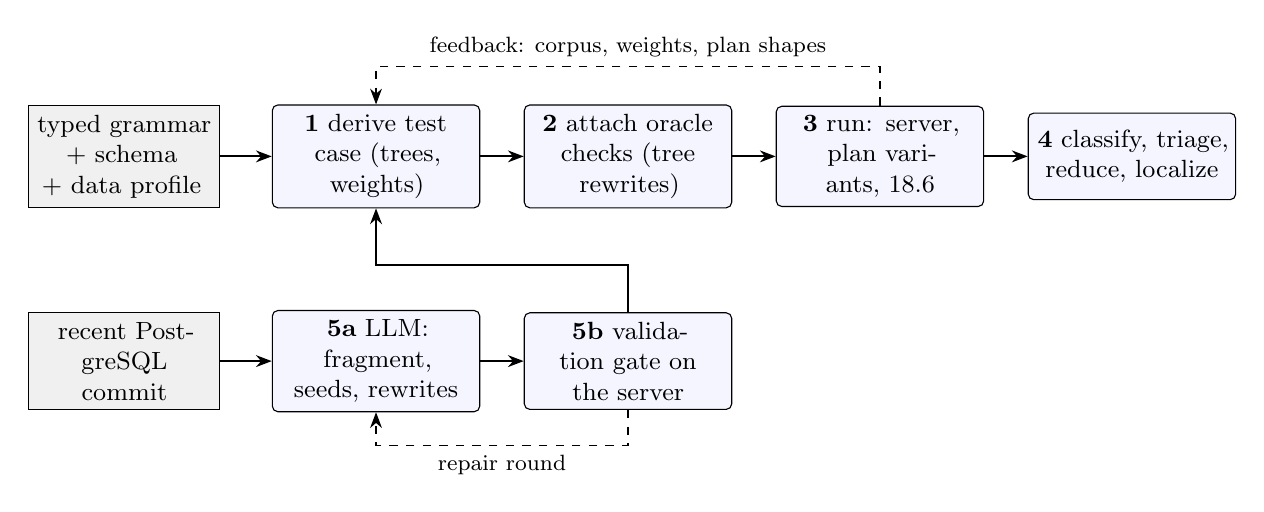
\begin{tikzpicture}[font=\small,
  box/.style={draw,rounded corners=2pt,align=center,fill=blue!4,minimum height=11mm,text width=24mm},
  io/.style={draw,align=center,fill=gray!12,minimum height=9mm,text width=22mm},
  fl/.style={-{Stealth[length=2mm]},thick}, bk/.style={-{Stealth[length=2mm]},dashed}]
\node[io] (g) at (0,0) {typed grammar\\+ schema\\+ data profile};
\node[box] (s1) at (3.2,0) {\textbf{1} derive test case (trees, weights)};
\node[box] (s2) at (6.4,0) {\textbf{2} attach oracle checks (tree rewrites)};
\node[box] (s3) at (9.6,0) {\textbf{3} run: server, plan variants, 18.6};
\node[box] (s4) at (12.8,0) {\textbf{4} classify, triage, reduce, localize};
\node[io] (c) at (0,-2.6) {recent \pg commit};
\node[box] (s5) at (3.2,-2.6) {\textbf{5a} LLM: fragment, seeds, rewrites};
\node[box] (s6) at (6.4,-2.6) {\textbf{5b} validation gate on the server};
\draw[fl] (g)--(s1); \draw[fl] (s1)--(s2); \draw[fl] (s2)--(s3); \draw[fl] (s3)--(s4);
\draw[bk] (s3.north) -- ++(0,0.5) -| node[pos=0.25,above]{\footnotesize feedback: corpus, weights, plan shapes} (s1.north);
\draw[fl] (c)--(s5); \draw[fl] (s5)--(s6);
\draw[bk] (s6.south) -- ++(0,-0.45) -| node[pos=0.25,below]{\footnotesize repair round} (s5.south);
\draw[fl] (s6.north) -- ++(0,0.6) -| (s1.south);
\end{tikzpicture}
\caption{The fuzzing loop (top) and the LLM loop (bottom). Steps match Sections~\ref{sec:grammar}--\ref{sec:llm}.}
\end{figure}

\subsection{Repository map}

\begin{tabularx}{\linewidth}{lX}
\toprule
Path & Contents \\
\midrule
\file{src/grammar/postgres.pgg} & the typed grammar \\
\file{src/corpus/schema.sql, schema.yaml} & the 9-relation schema (SQL for the server, YAML for the generator) \\
\file{src/corpus/rls.sql, profile.json} & RLS policies; data profile \\
\file{src/pgfuzz/grammar/} & DSL parser (\file{dsl.py}), engine (\file{engine.py}), generator, rewriter (oracles), data profile, tree I/O \\
\file{src/pgfuzz/reference/} & \pg executor, cross-version executor \\
\file{src/pgfuzz/eval/} & oracle, differential digests and determinism filter, signatures, metrics, statistics, features, known-bug catalog \\
\file{src/pgfuzz/triage/} & tokenizer, token reduction, tree reduction, localization, triage driver, precision \\
\file{src/pgfuzz/llm/} & commit miner, prompts, client, gate, diff coverage, loop \\
\file{src/pgfuzz/bench/} & re-injected bug benchmark (verify, attribute) \\
\file{src/pgfuzz/runner/, runlog/, report/} & experiment runner, run logs, reports \\
\file{src/generator/} & the random/mutation arm (Stage 1) \\
\file{src/bench/reinjected/} & benchmark: 23 commits, PoCs, \file{bugs.yaml}, \file{verify.json} \\
\file{src/configs/} & \file{rq1.yaml}, \file{rq3.yaml}, hunt and local configs \\
\file{scripts/} & server builds and starts (\file{build_reinjected.sh}, \file{rq1_servers.sh}, \file{rq3_servers.sh}, \file{ref_server.sh}), bisection, setup \\
\file{triage/verdicts.yaml} & the verdict of every triaged candidate (feeds RQ2) \\
\file{docs/} & guides, plans, evidence, bug reports (\file{docs/bughunt/}), paper draft PDF \\
\file{paper/} & the ACM/FSE paper (LaTeX) \\
\bottomrule
\end{tabularx}

\subsection{One trial}

\texttt{python -m pgfuzz run configs/rq1.yaml -j 4} plans the trials (arm
$\times$ trial), and each worker runs one trial against its own server
(port = base port + worker). A trial loops: ask the generator for a test case,
execute it, classify the result, update metrics and the run log, save a
failure if the signature is new, give feedback to the generator. Per trial it
writes \file{manifest.json}, \file{events.jsonl}, \file{timeline.jsonl}
(snapshots every 30 s), \file{failures/<signature>/} and \file{summary.json}.
Trials are resumable: re-running the command skips finished trials. The seed of
trial $k$ is the same in every arm (paired design).

\section{Step 1: the typed grammar and the generator}
\label{sec:grammar}

\subsection{The \texttt{.pgg} format}

\begin{itemize}
  \item \texttt{\%type int "int" num ord key \dots{} w=6} declares a SQL type,
    its classes (\texttt{num}, \texttt{ord}, \texttt{key}, \dots) and a weight.
  \item A rule has alternatives with weights \texttt{<4>}; terminals are
    keywords or quoted strings; \texttt{x?0.3} is optional with probability
    0.3; \texttt{x\{1,4/","\}} repeats 1--4 times separated by commas.
  \item Rules can be typed: \texttt{expr<T>}, \texttt{expr<int>},
    \texttt{expr<X:key>} (a type variable restricted to a class).
  \item Attributes: \texttt{@scope} opens a new name scope,
    \texttt{@set(agg\_ok)} sets a context flag (aggregates allowed),
    \texttt{\^{}} marks elements derived early (FROM before SELECT, so the
    select list can see the FROM's columns).
  \item Builtins (Python): \texttt{@col(T)} a visible column of type T,
    \texttt{@lit(T)} a literal, \texttt{@dlit(T)} a literal from the data of the
    compared column, \texttt{@table} a relation with a fresh alias,
    \texttt{@items} the select list, \texttt{@group\_keys} makes the level
    grouped, \texttt{@sorted\_agg} order-sensitive aggregates made
    deterministic, and about 20 more for DDL and DML.
\end{itemize}

A real excerpt:
\begin{lstlisting}
query @scope
  : <8> select_core order_by?0.3 limit_clause?0.06
  | <2> with_clause select_core order_by?0.2
  | <2> set_query
  ...
select_core
  : <6> SELECT distinct?0.12 @items ^from_clause ^where_clause?0.6
  | <3> SELECT @items ^from_clause ^where_clause?0.5 GROUP BY ^@group_keys having_clause?0.4
  | <2> SELECT @items ^from_clause ^where_clause?0.5 ^@global_agg having_clause?0.2
  ...
expr<bool>
  : <4> "(" expr<X:key> cmp expr<X> ")"
  | <1.2> "(" @col(X:ord) cmp @dlit(X) ")"
  | <2> "(" expr<bool> AND expr<bool> ")"
  | <1> "(" expr<X:key> NOT?0.3 IN "(" expr<X>{1,4/","} ")" ")"
  ...
\end{lstlisting}

Conventions that make oracles possible: every binary operator is
parenthesised (precedence never changes types); every column is qualified with
a unique alias; order-sensitive aggregates order by their own argument.

\subsection{The engine}

The engine expands a rule into a tree, choosing an alternative by weight,
binding type variables (\texttt{X}) consistently, tracking scopes (which
aliases and columns are visible, correlated or isolated) and flags (grouped
level, inside an aggregate). It backtracks when an alternative cannot be
completed (\texttt{Fail}) and prefers shallow alternatives past a soft depth.
Each alternative knows its minimal derivation depth (\texttt{mind}). While
rendering, each node's tokens are wrapped in invisible markers
(\verb|\x01<nid>| \dots{} \verb|\x02<nid>|), so the exact token span of every node
is known afterwards. A \texttt{MINIMAL} marker on a guide node makes the
engine derive that subtree with its smallest alternatives (used by tree
reduction).

\paragraph{Replay.} Given a guide tree, the engine follows its choices
(same alternatives, same columns, same literals), re-binding names and types
in the current schema state. Mutation and reduction both use replay, so their
results stay valid. Trees are stored with failures as JSON using stable
alternative \emph{ordinals} (uids are process-local) and exact container
types; 599 of 600 test cases replay to identical SQL in a fresh process.

\subsection{The generator}

\paragraph{A test case} is 0--2 setup statements (DDL such as
\texttt{CREATE INDEX}/\texttt{TABLE}, DML, \texttt{ANALYZE}, \texttt{SET LOCAL}
of a planner setting) followed by 1--2 queries or DML statements.

\paragraph{Fresh or mutated.} With probability 0.5 a corpus entry is picked
(weighted by its finds and how often it was picked) and mutated:
\emph{regen} (re-derive one subtree), \emph{splice} (graft a subtree from
another corpus entry), \emph{insert} (add a statement), \emph{drop} (remove one).

\paragraph{Corpus admission.} A test case enters the corpus if it produced a
new bug signature, a new SQL feature (catalogue of 148), a new pair of
features, or a new plan shape (digest of node types of
\texttt{EXPLAIN (FORMAT JSON, COSTS OFF)}).

\paragraph{Feedback-weighted alternatives} (plan 5.3). Each alternative has a
weight multiplier. After every test case, each alternative used in a tree gets
reward $r = 1$ if the test case entered the corpus, $-0.5$ if that tree's
statement failed, else 0; its weight is multiplied by $e^{\eta(r - \bar r)}$
with $\eta=0.1$ and $\bar r$ a running average, clipped to $[0.2, 5]$.
\emph{Measured:} 533 vs 419 distinct plan shapes in 1{,}000 test cases at the
same validity; the bandit learned to damp window-function alternatives that
often fail. RQ1 contains an ablation arm without it.

\paragraph{Data profile} (plan 6, interval and constraint-based analysis).
\texttt{pgfuzz profile} asks the server for min, max and the 10/25/50/75/90\%
quantiles of every column (\file{corpus/profile.json}). With probability 0.3 a
literal comes from it: boundary values (observed min$\pm$1, max$\pm$1, 0, $-0$,
NaN, $\pm$Infinity, the largest int, the empty array) or quantiles. The new
builtin \texttt{@dlit(T)} takes a quantile of the \emph{column the predicate
compares} (the engine remembers the last \texttt{@col}), so
\texttt{col < @dlit} selects a real share of rows. \emph{Measured:}
column-vs-constant predicates selecting 5--95\% of their table: 29.3\%
$\rightarrow$ 58.6\%.

\paragraph{Validity tuning loop.} \texttt{pgfuzz sample --execute} prints the
valid rate, the top error messages and the worst alternatives (by valid
rate); each fix is to one rule. This loop raised validity from 83\% to 100\%
before meeting 1.

\subsection{The schema}

Nine relations shared by both arms: \texttt{t0} (int, text, float8), \texttt{t1}
(int PK, int, jsonb, int4range), \texttt{t2} (identity bigint, numeric,
timestamptz, text[]), \texttt{t3} (int NOT NULL, bool, date, interval, int[],
text), \texttt{t4} (virtual and stored generated columns), \texttt{tp}
(range-partitioned), \texttt{tl} (list-partitioned), \texttt{ti} (inheritance
parent with child), \texttt{v0} (a view). Data is deterministic (no
\texttt{now()}), with NULLs in most columns. Indexes: B-tree (including
multi-column \texttt{t3(c0,c2)} for skip scan), GIN, GiST, BRIN, and an
expression index with a predicate.

\section{Steps 2--3: executing a test case and the oracles}
\label{sec:oracles}

A fuzzer is only as good as its oracle. This section explains every way the
system decides that \pg did something wrong, and, just as important, every
rule that stops it from calling correct behaviour a bug.

\begin{figure}[h]
\centering
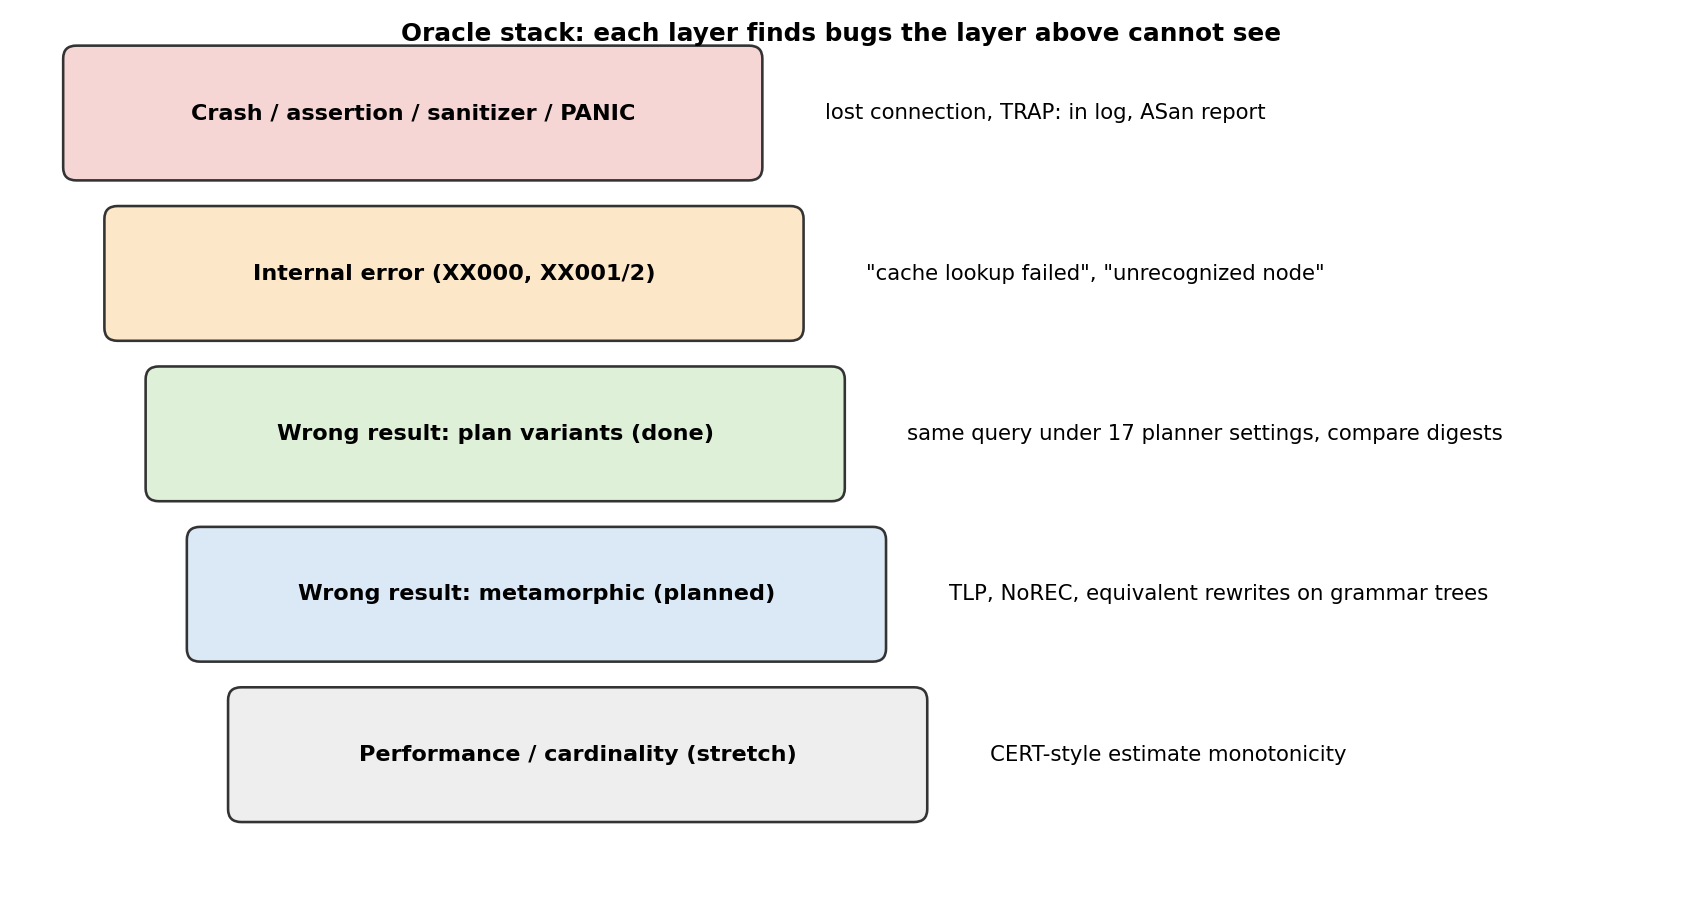
\includegraphics[width=0.85\linewidth]{oracle_stack.png}
\caption{The oracle stack: crash and error oracles see every statement;
plan-variant, metamorphic and cross-version oracles see deterministic queries.}
\end{figure}

\subsection{The executor}

\file{src/pgfuzz/reference/pg_executor.py} (741 lines) runs one test case on a
real server.
\begin{enumerate}
  \item \textbf{Isolation.} The test case runs inside one transaction; each
    statement in its own savepoint (\texttt{SAVEPOINT}, then \texttt{RELEASE} or
    \texttt{ROLLBACK TO}). At the end everything is rolled back, so the database
    is identical for the next test case. Statements that cannot run in a
    transaction (\texttt{VACUUM}, \texttt{CREATE INDEX CONCURRENTLY}) use
    \texttt{isolation: autocommit} plus a \texttt{reset\_sql} script.
  \item \textbf{Timeout} per statement (\texttt{statement\_timeout}, default 3 s
    in campaigns) so a slow plan cannot stall a worker.
  \item \textbf{Server log.} After each statement the executor reads new lines
    of the server log and looks for \texttt{TRAP:} (assertion),
    \texttt{PANIC:}, ``terminated by signal'', sanitizer reports and
    \texttt{BACKTRACE:} lines (\pg prints a C backtrace for internal errors
    when \texttt{backtrace\_on\_internal\_error = on}).
  \item \textbf{Crash recovery.} If the connection is lost, it waits for the
    postmaster to finish crash recovery (SQLSTATE 57P03 ``in recovery''),
    reconnects, and recreates the per-worker database if needed.
  \item \textbf{Digests.} For each successful query it computes an
    order-insensitive digest of the result (below) so it can compare results
    without storing them.
  \item \textbf{Oracle work} for each successful, deterministic query: plan
    variants, metamorphic checks, plan shape (\texttt{EXPLAIN (FORMAT JSON,
    COSTS OFF)} digest), optionally coverage sampling.
\end{enumerate}

\paragraph{Foreign-crash filter.} When one backend crashes, \pg restarts
\emph{all} backends; every other session sees ``terminating connection because
of crash of another server process'' (57P02). Each worker has its own server,
but our own manual PoC replay once crashed a server that a campaign was using
and the random arm was blamed. Now the executor records its backend PID
(\texttt{pg\_backend\_pid()}); crash evidence in the log must name that PID
(or a parallel worker of our own query), otherwise the event is classified
as \emph{foreign} and ignored (\texttt{\_foreign\_crash}).

\subsection{Classification}
\label{sec:classify}

\file{src/pgfuzz/eval/oracle.py} turns executor facts into one
\texttt{Outcome}, in priority order:
\begin{enumerate}
  \item log evidence: assertion, sanitizer, signal (crash), \texttt{PANIC};
  \item connection loss without an orderly SQLSTATE: crash;
  \item the SQLSTATE of a failing statement, by class:
    42601 $\rightarrow$ syntax; 42, 0A, 25, \dots{} $\rightarrow$ semantic;
    22, 23 \dots{} $\rightarrow$ runtime; 57014 $\rightarrow$ timeout;
    53, 54 $\rightarrow$ resource limit; \textbf{XX000 $\rightarrow$ internal
    error}; XX001/XX002 $\rightarrow$ data corruption. A short list of XX000
    messages that are really resource exhaustion (``out of memory'' in a
    hash table, etc.) is demoted;
  \item plan-variant facts: a variant that raised an internal error, or
    returned a different digest $\rightarrow$ \texttt{wrong\_result} (variant
    name recorded);
  \item metamorphic facts: a \emph{confirmed} mismatch $\rightarrow$
    \texttt{wrong\_result} with variant \texttt{mm:<kind>}; a CERT violation
    $\rightarrow$ \texttt{performance} (not a wrong answer).
\end{enumerate}
The outcomes are ordered by severity (ok $<$ syntax $<$ semantic $<$ runtime
$<$ timeout $<$ resource $<$ terminated $<$ performance $<$ wrong result $<$
internal error $<$ corruption $<$ panic $<$ assertion $<$ sanitizer $<$ crash).
The test case gets the most severe statement outcome; the index of that
statement is the \emph{culprit}. Bug candidates are: crash, assertion,
sanitizer, panic, corruption, internal error, wrong result, and (reported
separately) performance.

\subsection{Determinism: which queries may be compared at all}
\label{sec:eligible}

Comparing two runs of a query only makes sense if the correct answer is a
single multiset. \texttt{eligible(sql)} in \file{src/pgfuzz/eval/differential.py}
accepts a statement only if:
\begin{itemize}
  \item it is \texttt{SELECT}, \texttt{VALUES} or \texttt{TABLE} and contains no
    \texttt{INSERT/UPDATE/DELETE/MERGE/INTO} (no side effects);
  \item no \texttt{LIMIT}, \texttt{OFFSET}, \texttt{FETCH}, \texttt{TABLESAMPLE},
    \texttt{DISTINCT ON}, \texttt{FOR UPDATE/SHARE}, \texttt{SKIP LOCKED}
    (all choose \emph{some} rows, and which ones depends on the plan);
  \item no volatile function (\texttt{random}, \texttt{clock\_timestamp},
    \texttt{nextval}, \texttt{gen\_random\_uuid}, \texttt{pg\_sleep}, \dots, 42 names);
  \item no order-dependent window function (\texttt{row\_number}, \texttt{ntile},
    \texttt{lag/lead}, \texttt{first/last/nth\_value}) and no \texttt{ROWS}
    frame (ties are broken by the plan); \texttt{rank}, \texttt{dense\_rank},
    \texttt{percent\_rank}, \texttt{cume\_dist} are tie-safe and allowed;
  \item no order-sensitive aggregate without its own \texttt{ORDER BY}:
    \texttt{array\_agg}, \texttt{string\_agg}, \texttt{json(b)\_agg},
    \texttt{json(b)\_object\_agg}, \texttt{xmlagg}, \texttt{json\_arrayagg},
    \texttt{json\_objectagg}, \texttt{any\_value}, \dots;
  \item no \texttt{ARRAY(SELECT \dots)} without \texttt{ORDER BY} inside
    (added after candidate~1 of the bug hunt, a false positive).
\end{itemize}
The grammar helps: \texttt{@sorted\_agg} writes \texttt{array\_agg(x ORDER BY
x)}, so most aggregates the generator emits \emph{are} eligible.

\subsection{Result digests}
\label{sec:digest}

All values are fetched as text (\pg's own output format) and canonicalised:
\begin{itemize}
  \item \textbf{numeric scale:} \texttt{2.0}, \texttt{2.00} $\rightarrow$
    \texttt{2} (equal values; \texttt{DISTINCT}/\texttt{GROUP BY}/\texttt{UNION}
    may legitimately keep either representative -- found as a false positive in
    smoke run~1);
  \item \textbf{float $-0$:} $-0$ and $0$ compare equal, so either may survive;
  \item \textbf{float masking:} if the query has a floating-point aggregate or
    window (\texttt{sum}, \texttt{avg}, \texttt{stddev}, \texttt{corr},
    \texttt{regr\_*}, \texttt{percentile\_cont}, \texttt{OVER}), float columns
    are reduced to a class: \texttt{NaN}, \texttt{Infinity},
    \texttt{-Infinity} or ``finite''. Summation order changes the last digits
    legitimately; it cannot turn a finite value into NaN. (Masking
    \emph{everything} at first hid a re-injected bug: 0 vs NaN. That is why
    the class is kept.)
\end{itemize}
Rows are joined with separator bytes, sorted (multiset semantics), and hashed
with BLAKE2b (96 bits). Results above 10{,}000 rows are not compared.

\subsection{Oracle 1: plan variants (differential testing inside one server)}
\label{sec:variants}

The same query is re-run with \texttt{set\_config(name, value, true)} (local to
a savepoint, rolled back) under planner configurations. The settings change
\emph{how} \pg runs the query, never \emph{what} it returns, so any digest
difference is a bug (given eligibility). The 18 variants:

\begin{center}
\small
\begin{tabularx}{\linewidth}{lX}
\toprule
Variant & Settings (what it forces) \\
\midrule
\texttt{nestloop\_only} & hash and merge join off \\
\texttt{hashjoin\_only} & nested loop and merge join off \\
\texttt{mergejoin\_only} & nested loop and hash join off \\
\texttt{no\_hashagg} & sort-based grouping \\
\texttt{no\_sort\_opt} & no incremental sort, no presorted aggregate \\
\texttt{index\_scans} & seq scan and bitmap scan off \\
\texttt{seq\_scans} & index, index-only and bitmap scans off \\
\texttt{no\_memoize\_material} & no Memoize, no Material nodes \\
\texttt{parallel} & \texttt{debug\_parallel\_query=on}, zero parallel costs, 4 workers, leader not participating \\
\texttt{partitionwise} & partition-wise join and aggregate on \\
\texttt{no\_partition\_pruning} & partition pruning off \\
\texttt{geqo} & genetic optimizer from 2 relations \\
\texttt{no\_join\_reorder} & \texttt{join/from\_collapse\_limit = 1} (syntactic join order) \\
\texttt{tiny\_work\_mem} & \texttt{work\_mem=64kB}: hash joins batch, sorts spill to disk \\
\texttt{no\_reordering} & no GROUP BY / DISTINCT key reordering (PG 17/18 features) \\
\texttt{no\_self\_join\_elim} & self-join elimination off (new in PG 18) \\
\texttt{no\_eager\_agg} & eager aggregation off (new on master, Oct 2026) \\
\texttt{jit} & JIT compile everything (costs 0) \\
\bottomrule
\end{tabularx}
\end{center}

Settings unknown to the server are dropped at start (each variant is probed
once), so the same config works on 17, 18.6 and master. To keep throughput,
each query runs under \texttt{per\_query = 2} variants chosen
deterministically from a hash of the SQL text (\texttt{pick\_variants}): a
failure replays with the same variant, and over a campaign every variant is
used. A failure is \emph{materialised} for reports: the culprit statement is
preceded by explicit \texttt{SET} commands of the variant.

\paragraph{Why this finds bugs.} Each variant forces the planner down a
different code path (another join method, another aggregation strategy, a
parallel plan, spilling). Many optimizer bugs live in exactly one path.
Re-injected bug \texttt{rb-dfcf6fa7} was found this way in smoke run~2.

\subsection{Oracle 2: metamorphic rewrites of the derivation tree}
\label{sec:mm}

\file{src/pgfuzz/grammar/rewrite.py} (656 lines). For each eligible query, the
rewriter looks at its \emph{derivation tree} and the token span of each node,
and builds up to \texttt{per\_query} checks. A check has a left side (the
original query, or a variant of it) and a right side (the rewritten query);
both must return the same multiset. Kinds are sampled by weight (partition
checks apply to fewer queries, so they get larger weights: TLP-WHERE 6,
TLP-HAVING 5, TLP-agg 5, NoREC 3, expression 3, predicate 3, RLS 2, NOT NULL
1.5, CTE 1.5, fence 1.5, ORDER BY 1, CERT 1).

\begin{keybox}[Why do this on a tree and not on a string?]
SQLancer builds its own small queries so it knows their structure. We have
arbitrary, deeply nested queries from a 421-alternative grammar. The tree tells
us exactly which tokens are the \texttt{WHERE} predicate of \emph{this}
\texttt{SELECT} (not of a subquery), which expression has which type, which
level is grouped, which columns are in scope, and whether a node sits under an
outer join. A string rewrite would have to re-parse SQL and would get all of
these wrong some of the time; each mistake is a false positive.
\end{keybox}

\paragraph{Where a rewrite may apply.} Partition checks (TLP) apply to any
\texttt{select\_core} whose result is used as a multiset by the enclosing
query: the query itself, a subquery in \texttt{FROM}, a set-operation arm, an
\texttt{IN}/\texttt{EXISTS} subquery, a \texttt{LATERAL} subquery
(\texttt{MULTISET\_CONTEXTS}). Replacing a multiset by an equal multiset cannot
change the statement. A scalar subquery is \emph{not} such a context (it must
return one row), so it is not partitioned. Levels with window functions are
skipped (a window sees the whole partition; splitting the rows changes it).

\subsubsection*{The twelve kinds}

\begin{longtable}{p{0.17\linewidth}p{0.42\linewidth}p{0.33\linewidth}}
\toprule
\textbf{Kind} & \textbf{Rewrite (left $\equiv$ right)} & \textbf{Soundness conditions / targets} \\
\midrule
\endhead
\texttt{tlp\_where} & \texttt{SELECT .. FROM f} $\equiv$ \texttt{(.. WHERE p) UNION ALL (.. WHERE NOT p) UNION ALL (.. WHERE p IS NULL)} & Ternary logic partition (Rigger \& Su 2020). Not grouped. With \texttt{DISTINCT}: \texttt{UNION} instead, and only if all output types have a unique text form. Nested arms parenthesised so \texttt{INTERSECT} cannot regroup them. \\
\texttt{tlp\_having} & \texttt{.. GROUP BY k HAVING TRUE} $\equiv$ union of \texttt{HAVING p}, \texttt{NOT p}, \texttt{p IS NULL} & Grouped levels; group keys must have unique text form. Left side keeps \texttt{HAVING TRUE}: removing \texttt{HAVING} from a level without \texttt{GROUP BY} changes it from a one-group aggregate to a plain query (our false positive in smoke run~1). \\
\texttt{tlp\_agg} & \texttt{SELECT MIN(e) AS c0, COUNT(x) AS c1 FROM f} $\equiv$ \texttt{SELECT MIN(t.c0), SUM(t.c1) FROM (three partitions) t} & TLP for aggregates. Only combinable aggregates: MIN, MAX, SUM, COUNT$\rightarrow$SUM, BIT\_AND/OR/XOR, BOOL\_AND/OR, EVERY; no DISTINCT, FILTER or ORDER BY inside; every item exactly one call. \\
\texttt{norec} & \texttt{SELECT COUNT(*) FROM f WHERE p} $\equiv$ \texttt{SELECT COALESCE(SUM(CASE WHEN p THEN 1 ELSE 0 END),0) FROM f} & NoREC (Rigger \& Su 2020): the optimizer can use \texttt{p} in the first form (index, pushdown, join pruning) but must evaluate it per row in the second. \\
\texttt{expr} & replace one typed expression node $e$ by an equal one: \texttt{CASE WHEN TRUE THEN e END}, \texttt{COALESCE(e,e)}, \texttt{(SELECT e)}, \texttt{e+0}, \texttt{e*1}, \texttt{e||''}, \texttt{NOT NOT e}, \texttt{e AND TRUE}, \texttt{e OR FALSE}, \texttt{CASE WHEN e THEN TRUE WHEN NOT e THEN FALSE END} & EET-style (Jiang \& Su 2024). Rewrites are chosen \emph{by the node's type} (\texttt{+0} on float8 is excluded: $-0+0$ prints 0). No rewrite inside aggregates/windows for \texttt{(SELECT e)}. \textbf{\texttt{scalar\_sub} found BUG-02.} \\
\texttt{pred:in\_or} & \texttt{e IN (a,b)} $\equiv$ \texttt{(e=a) OR (e=b)} (also \texttt{NOT IN}) & Targets PG 18's OR-to-\texttt{= ANY} transformation. \\
\texttt{pred:cmp\_negate} & \texttt{a < b} $\equiv$ \texttt{NOT (a >= b)} & Exact under 3-valued logic for types with a B-tree total order. \\
\texttt{pred:between} & \texttt{x BETWEEN lo AND hi} $\equiv$ \texttt{x >= lo AND x <= hi} & Range/index-condition code. \\
\texttt{notnull} & \texttt{WHERE p} $\equiv$ \texttt{WHERE (p AND c IS NOT NULL)} for a NOT NULL column $c$ that $p$ already uses & Targets NOT-NULL-based simplification (PG 18). Not under outer joins (NULL-extended columns); not generated columns; $c$ must be in the scope of the predicate, not of a nested sub-select (\texttt{\_nested\_under}; a bug we fixed). \\
\texttt{order\_drop} & remove the statement's own \texttt{ORDER BY} & Multiset unchanged (no LIMIT, by eligibility). Exercises sort elimination and incremental sort. \\
\texttt{cte\_materialize} & \texttt{WITH x AS (..)} $\leftrightarrow$ \texttt{AS MATERIALIZED (..)} $\leftrightarrow$ \texttt{AS NOT MATERIALIZED} & Inlining vs materialisation of CTEs. \\
\texttt{table\_fence} & \texttt{t AS a} $\equiv$ \texttt{(SELECT * FROM t OFFSET 0) AS a} & \texttt{OFFSET 0} is an optimisation fence: no pull-up, no pushdown into the table. \\
\texttt{rls} & see below & information-flow oracle \\
\texttt{cert} & see below & performance oracle \\
\bottomrule
\end{longtable}

\paragraph{Example (TLP-WHERE), generated and rewritten by the tool:}
\begin{lstlisting}
-- original (left side keeps everything except WHERE)
SELECT t0_1.c0 AS c0 FROM t0 AS t0_1
-- right side
(SELECT t0_1.c0 AS c0 FROM t0 AS t0_1 WHERE ((t0_1.c0 > 5)))
UNION ALL
(SELECT t0_1.c0 AS c0 FROM t0 AS t0_1 WHERE NOT ((t0_1.c0 > 5)))
UNION ALL
(SELECT t0_1.c0 AS c0 FROM t0 AS t0_1 WHERE ((t0_1.c0 > 5)) IS NULL)
\end{lstlisting}

\paragraph{Confirmation.} A first mismatch is not enough: both sides are run
again. Only if both re-runs return the same digests as the first runs is the
mismatch \emph{confirmed}; otherwise it is \emph{unconfirmed} (the query is
not deterministic after all) and ignored. Errors on one side (``side errors'',
for example a rewrite that overflows) are counted, not reported, unless they are
internal errors.

\paragraph{LLM-proposed rewrites} come in as templates such as
\texttt{COALESCE(\{e\}, \{e\})} with a type; they are added to the same
\texttt{expr} pool after passing the rewrite gate (Section~\ref{sec:rwgate}).

\subsection{Oracle 3: the RLS leak oracle (information flow)}
\label{sec:rls}

\paragraph{Setup.} \file{src/corpus/rls.sql} creates role \texttt{pgfuzz\_rls}
(SELECT on all tables) and one policy on five tables:
\texttt{t0}: \texttt{(c0 \% 3) <> 0};
\texttt{t1}: \texttt{c1 IS NULL OR c1 < 30};
\texttt{t3}: \texttt{c1 IS NOT FALSE};
\texttt{tp}: \texttt{c0 > 10};
\texttt{ti}: \texttt{c1 IS DISTINCT FROM 'a'}.
The executor connects as a superuser, which bypasses RLS, so these policies
change nothing for the other oracles. As the role, 131 of the 203 rows of
\texttt{t0} are visible.

\paragraph{The check.} Left: the original query run with \texttt{SET LOCAL
ROLE pgfuzz\_rls} (policies apply). Right: the query run as superuser with
every protected table reference \texttt{t AS a} replaced by
\texttt{(SELECT * FROM t WHERE (policy)) AS a}. Both must be equal. A left side
with \emph{more} rows means a \textbf{leak}: the restricted role saw a row the
policy hides -- for example because a leaky function or an operator was pushed
below the security barrier, or a plan path forgot the policy qual. Fewer rows
means a wrong result.

\paragraph{Why it matters.} It connects the project to the course's
information-flow lectures (L21--22): the policy is a confidentiality label; the
oracle checks non-interference on concrete data. RLS bugs are security bugs
(\pg has had CVEs in this area, e.g. CVE-2023-2455 and CVE-2024-10976).
\emph{Measured:} 532 live checks on master, 0 false positives.

\subsection{Oracle 4: CERT (cardinality-estimation restriction testing)}
\label{sec:cert}

CERT (Ba \& Rigger, ICSE 2024): adding a restriction to a query must not
\emph{increase} the planner's row estimate. Left: \texttt{EXPLAIN} of the query
without its \texttt{WHERE}; right: \texttt{EXPLAIN} of the query. If the
estimate of the restricted query exceeds the unrestricted one, the outcome is
\texttt{performance} (a bad estimate leads to bad plans, but not to wrong
results). Restricted to ungrouped, non-\texttt{DISTINCT}, window-free levels,
where the monotonicity really holds. \emph{Measured:} 58 checks, 0 violations.
We report these separately and do not count them as wrong results.

\subsection{Oracle 5: cross-version (master vs 18.6)}
\label{sec:xversion}

\file{src/pgfuzz/reference/xversion_executor.py}. Every test case runs on the
server under test (master, assertions on) and on a reference (18.6 release).
For each statement that succeeded on both and is \texttt{xversion\_eligible},
the digests are compared; a difference is reported as a wrong result with
variant \texttt{xversion}, through the same path as plan variants.

\begin{itemize}
  \item \textbf{Why:} a new optimisation that is wrong under \emph{every}
    planner setting (no GUC turns it off) is invisible to plan variants but
    disagrees with a release that does not have it. Regressions in unreleased
    code are also what upstream fixes fastest (``open items'' before a
    release).
  \item \textbf{Exclusions:} clock and instance functions (\texttt{now},
    \texttt{current\_timestamp}, \texttt{version}, \texttt{pg\_backend\_pid},
    \texttt{current\_setting}, \dots) and functions whose behaviour changed
    \emph{on purpose}: \texttt{corr}, \texttt{regr\_r2/slope/intercept}
    (master commit \texttt{649828769} keeps $S_{xx}$ exactly 0 for constant
    input, so \texttt{corr(x,x)} over equal values is NULL on master, 1 on 18).
    We found that difference in smoke run~2 and confirmed it in the commit log.
  \item \textbf{Sequences} are not transactional: a \texttt{prelude\_sql}
    resets identity sequences on both servers before every test case.
  \item \textbf{Per-worker reference databases} \texttt{ref\_<worker>}, created
    by the executor (\texttt{create\_database}): four workers sharing one
    reference database raced on schema setup in smoke run~1.
  \item Statements that fail on only one side are counted
    (\texttt{test\_only\_ok}, \texttt{ref\_only\_ok}: new features, new errors)
    but not reported.
\end{itemize}
\emph{Measured:} 1{,}155 comparisons, 0 mismatches after the fixes.

\subsection{Signatures (deduplication)}
\label{sec:signatures}

Thousands of failing test cases may share one root cause. Each candidate gets
a signature (\file{src/pgfuzz/eval/signature.py}), strongest first:
\begin{description}
  \item[stack] top 5 symbolised frames of the backtrace, generic frames
    (\texttt{abort}, \texttt{ExceptionalCondition}, \texttt{PostgresMain},
    \dots) removed;
  \item[assert] assertion expression + source file;
  \item[message] SQLSTATE + error message with literals, numbers and hex
    abstracted (\texttt{N}, \texttt{?}, \texttt{H});
  \item[diff] for wrong results: oracle/variant + verb and SQL features of the
    culprit statement;
  \item[weak] crash without stack: signal + statement shape.
\end{description}
A failure directory is written only for the first test case of each new
signature. ``Unique bug candidates'' in the results are counted by signature,
and the strength is logged, because signature quality is a threat to validity.

\section{Step 4: triage -- from a failure to a bug report}
\label{sec:triage}

A campaign produces failure directories (one per new signature). Most
candidates are not reportable as they are: test cases are long, some are
flaky, some are our own false positives. \texttt{python -m pgfuzz triage
<config> <failure dir>} (\file{src/pgfuzz/triage/triage.py}) turns a candidate
into either a verdict \emph{flaky} or a reduced reproducer with a draft report.

\begin{center}
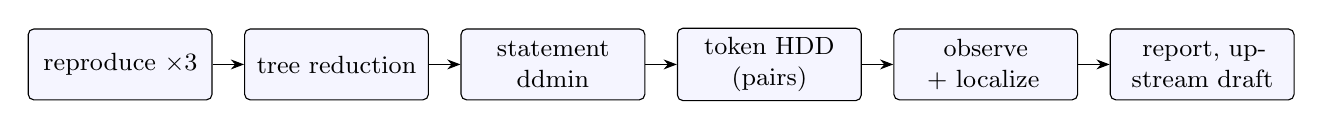
\begin{tikzpicture}[font=\small, node distance=4mm,
  b/.style={draw,rounded corners=2pt,fill=blue!4,align=center,minimum height=9mm,text width=21mm}]
\node[b] (a) {reproduce $\times 3$};
\node[b,right=of a] (b) {tree reduction};
\node[b,right=of b] (c) {statement ddmin};
\node[b,right=of c] (d) {token HDD (pairs)};
\node[b,right=of d] (e) {observe + localize};
\node[b,right=of e] (f) {report, upstream draft};
\foreach \x/\y in {a/b,b/c,c/d,d/e,e/f} \draw[-{Stealth}] (\x)--(\y);
\end{tikzpicture}
\end{center}

\subsection{Reproduce}

The candidate is executed three times by the \emph{same executor and oracle}
as the campaign, configured for its oracle: only the failing plan variant, or
only its metamorphic check (with confirmation on). \texttt{same\_failure}
decides whether a re-run shows \emph{the same} failure, not just any failure:
\begin{itemize}
  \item assertion: same file and same expression;
  \item wrong result: same variant / oracle kind;
  \item internal error, corruption, panic: same normalised message;
  \item crash without assertion: any crash of the same statement.
\end{itemize}
0/3 $\Rightarrow$ verdict \emph{flaky}, nothing else is done (2 of our 18
candidates). This criterion is also what every reduction step uses.

\subsection{Reduction, three levels}
\label{sec:reduce}

\paragraph{1. Tree reduction} (\file{src/pgfuzz/triage/tree_reduce.py}) -- the
fourth job of the derivation tree. The failure directory stores the trees of
the test case (JSON, stable alternative ordinals). Moves, biggest expected gain
first:
\begin{enumerate}
  \item drop a whole statement;
  \item drop one element of a repetition (\texttt{\#rep});
  \item replace a subtree by the \emph{smallest derivation of the same rule and
    type}: the node is replaced by a \texttt{MINIMAL} marker and the engine
    derives it with its minimal-depth alternatives.
\end{enumerate}
After each move the generator \emph{replays} the trees (re-binding names,
aliases and types), so almost every candidate is valid SQL: the server's time
goes to the question that matters (does the failure remain?), not to rejecting
broken SQL. A candidate is only tried if it is smaller in tokens; after each
success the search restarts from the biggest moves.

\paragraph{2. Statement ddmin} (\texttt{reduce\_statements}): remove setup
statements that are not needed (Zeller \& Hildebrandt's delta debugging),
always keeping the culprit.

\paragraph{3. Token HDD} (\texttt{TokenReducer}, \file{reduce.py}): hierarchical
delta debugging over the \emph{parenthesis tree} of the culprit statement
(Misherghi \& Su). Coarse passes first: remove a clause (\texttt{WHERE},
\texttt{ORDER BY}, \dots), remove one list element, unwrap a parenthesised
sub-expression or replace it by a small literal (\texttt{NULL}, \texttt{1},
\texttt{TRUE}, \texttt{FALSE}, \texttt{0}, \texttt{''}); then single tokens.
Results are cached by text; budget 500 tests or 15 minutes.

\paragraph{Pairs.} For a metamorphic candidate (query $Q$ and rewrite $Q'$)
both sides must stay equivalent while being reduced. \texttt{split\_pair}
computes the common prefix and suffix of the two token lists and leaves a
\texttt{HOLE} where they differ; the reducer edits the shared skeleton, and both
sides are materialised by filling the hole with each side's middle. So every
edit is applied to both sides at once and the hole is never removed.

\begin{keybox}[Measured: tree reduction vs token reduction (BUG-01)]
A real grammar test case failing BUG-01's assertion: 3 statements, 590 tokens.
\begin{center}
\begin{tabular}{lrrr}
\toprule
Reduction & Final culprit & Server runs & Time \\
\midrule
statements + tokens only (\texttt{--no-tree}) & 116 tokens & 406 & 33.7 s \\
tree first, then statements + tokens & \textbf{79 tokens} & 555 & 39.6 s \\
\bottomrule
\end{tabular}
\end{center}
The tree stage alone: 590 $\rightarrow$ 136 tokens in 150 runs (196 replays).
Token reduction gets stuck in local minima (removing any single token breaks
the SQL); the tree can jump to a \emph{different, smaller} valid derivation.
Evidence: \file{docs/evidence/tree_reduction/}. BUG-02's first candidate:
4 statements / 107 tokens $\rightarrow$ 1 statement / 36 tokens in 307 runs
(token level, before tree reduction existed).
\end{keybox}

\subsection{Observe and localize}
\label{sec:localize}

After reduction, triage runs the queries to show (both sides for a pair, or
the query under default and failing settings) and records up to 30 result rows
on the test server and, if configured, on the 18.6 reference.

Then \file{src/pgfuzz/triage/localize.py} combines the two oracle families
(plan section~0.3 ``plan oracle $\times$ rewrite oracle''): it re-runs the
reduced queries under \emph{every} plan variant and reports, per variant, whether
the answer changes and whether the two sides agree. Verdicts:
\begin{description}
  \item[planner] the disagreement disappears when some settings are switched
    off: those code paths are the first suspects. A table
    (\texttt{SUSPECTS}) maps each setting to source files, e.g.
    \texttt{enable\_hashjoin} $\rightarrow$ \file{executor/nodeHashjoin.c,
    optimizer/path/joinpath.c}; \texttt{enable\_eager\_aggregate}
    $\rightarrow$ \file{optimizer/path/allpaths.c, optimizer/util/relnode.c}.
  \item[not toggled by planner settings] no setting removes it: suspect an
    always-applied rewrite, constant folding, a planner support function or
    expression evaluation. \textbf{BUG-02 is localized this way}, and its true
    cause is exactly a planner support function (\texttt{rangetypes.c}).
  \item[sides agree by default] the reduction went wrong (a warning).
\end{description}

\subsection{Outputs}

Per candidate, in \file{results/triage/<signature>/}:
\begin{itemize}
  \item \file{reduced.sql}: setup statements, then the culprit; for plan
    variants the \texttt{SET} commands are written out; for metamorphic
    candidates both queries, so the file is a stand-alone reproducer for
    \texttt{psql};
  \item \file{triage.json}: reproduction counts, sizes before/after, runs,
    seconds, observed rows, localization, server versions;
  \item \file{report.md}: a readable report;
  \item \file{upstream_report.txt}: a draft for the \texttt{pgsql-bugs} form,
    in the shape \pg developers expect (version and build, what happens, the
    minimal script, actual output on master and on the release, the
    localization, the top 12 backtrace frames, and two placeholders we must
    fill by hand: \emph{expected behaviour with a justification from the SQL
    standard or the documentation}, and the bisected commit).
\end{itemize}
The tool never writes the ``expected'' part: deciding that something is a bug
is a human judgement.

\paragraph{Bisection.} \file{scripts/bisect_pg.sh GOOD BAD reduced.sql MODE}
runs \texttt{git bisect} on a full-history \pg clone, building each step into a
scratch prefix. Modes: \texttt{crash} (backend crash or assertion),
\texttt{error} (psql reports an ERROR), \texttt{output} (differs from an expected
output), \texttt{differ} (the last two queries of \file{reduced.sql} return
different rows -- for metamorphic and plan-variant candidates). Commits that do
not build are skipped (exit 125).

\section{The precision ledger (RQ2 and claim 2)}
\label{sec:ledger}

Every triaged candidate gets an entry in \file{triage/verdicts.yaml}: signature,
oracle, verdict (\emph{real, duplicate, false\_positive, not\_a\_bug, flaky}),
a note, \texttt{fixed: true} if the false-positive class has been fixed in the
tool, and the upstream link. \texttt{python -m pgfuzz precision} computes
(\file{src/pgfuzz/triage/precision.py}):
\[
\text{precision} = \frac{\text{real}}{\text{real} + \text{false positive} + \text{not a bug}},
\qquad
\text{after fixes} = \frac{\text{real}}{\text{decided} - \text{fixed}}.
\]
Duplicates count towards neither side; flaky entries are reported separately.

\paragraph{The ledger today (18 candidates).}
\begin{center}
\small
\begin{tabular}{lrrrrrr}
\toprule
Oracle & Candidates & Real & False pos. & Duplicates & Precision & After fixes \\
\midrule
assertion & 2 & 1 & 1 & 0 & 0.50 & 1.00 \\
crash & 1 & 0 & 1 & 0 & 0.00 & -- \\
cross-version & 3 & 0 & 2 & 0 & 0.00 & -- \\
internal\_error & 2 & 1 & 0 & 0 & 1.00 & 1.00 \\
metamorphic:expr & 1 & 1 & 0 & 0 & 1.00 & 1.00 \\
metamorphic:tlp\_having & 4 & 0 & 4 & 0 & 0.00 & -- \\
plan-variant & 5 & 0 & 5 & 0 & 0.00 & -- \\
\midrule
all & 18 & 3 & 13 & 0 & 0.19 & 1.00 \\
\bottomrule
\end{tabular}

\end{center}

\begin{center}
\scriptsize
\begin{longtable}{p{0.16\linewidth}p{0.17\linewidth}p{0.12\linewidth}p{0.47\linewidth}}
\toprule
Signature & Oracle & Verdict & Note \\
\midrule
\endhead
\rows{ledger_rows.tex}
\bottomrule
\end{longtable}
\end{center}

\paragraph{How to read it (be ready for this question).}
\begin{itemize}
  \item The 3 real ones: BUG-01 (assertion), BUG-02 (metamorphic expression
    rewrite), and the re-injected benchmark bug \texttt{rb-dfcf6fa7} (internal
    error), which counts as real because it is a real historical \pg bug, put
    back on purpose.
  \item 13 false positives / not-a-bug come from \textbf{6 classes}, all fixed
    in the tool with a test: (1) \texttt{ARRAY(SELECT)} without
    \texttt{ORDER BY} (5 plan-variant candidates); (2) clock-dependent seed
    data across versions; (3) TLP-HAVING without \texttt{GROUP BY} (4);
    (4) \texttt{DISTINCT} over numeric scale; (5) the shared-server PoC replay
    (2, assertion + crash); (6) the intended \texttt{corr} change (not a bug).
  \item Raw precision 0.19 is low \emph{on purpose}: we log every false
    positive we ever produced, including during development. ``After fixes''
    1.00 means every remaining decided report of a class we have not fixed was
    real. The paper reports both and the per-oracle counts of the long
    campaigns, which will be the honest number.
  \item The 798 new-kind checks, the 532 RLS checks, the 58 CERT checks and the
    1{,}991 metamorphic checks of the full-system smoke produced 0 new false
    positives.
\end{itemize}

\section{Step 5: the LLM arm -- the LLM proposes, the server decides}
\label{sec:llm}

\subsection{Why an LLM at all, and why this way}

The grammar knows the SQL we wrote rules for. \pg master gets new planner
features every few weeks (self-join elimination, eager aggregation, skip scan,
OR-to-\texttt{ANY}, NOT NULL simplification, \dots). Writing grammar for each by
hand is slow, and the newest code is where regressions are. An LLM can read a
commit (message, diff, the regression test it adds) and write grammar for it.

Two designs we rejected:
\begin{itemize}
  \item \textbf{LLM as the generator} (Fuzz4All style): one model call per
    test case is 1{,}000$\times$ slower than our 17--23 test cases per second,
    and the output is unchecked text with no derivation tree (so no oracles, no
    tree reduction).
  \item \textbf{LLM as the oracle} (``is this result correct?''): LLMs cannot
    evaluate SQL on our data reliably; every hallucinated ``bug'' costs triage
    time.
\end{itemize}
Our design keeps the model \emph{off the hot path}: a few calls per commit
produce a grammar fragment; the grammar then generates thousands of
variations, each a typed tree the oracles can use. And nothing the model writes
is trusted: a gate on the real server decides.

\subsection{The pipeline}

\begin{enumerate}
  \item \textbf{Mine} (\file{src/pgfuzz/llm/commits.py}):
    \texttt{pgfuzz llm mine <pg clone> --since 2026-06-29 --until 26bd08fb
    --exclude bench/reinjected/commits.txt}. Keeps commits that touch
    query-processing code (optimizer, executor, parser, \file{utils/adt},
    rewrite, nodes, \dots) and skips typo/comment/pgindent/revert/warning
    commits. For each it stores a \texttt{CommitDigest}: sha, date, subject,
    body, files, changed function names, the SQL lines it added to the
    regression tests, and the \textbf{diff-coverage targets} (changed line
    numbers of every \texttt{.c} file).
  \item \textbf{Prompt} (\file{prompt.py}). A system prompt that is the same for
    every commit and therefore \textbf{cached} ($\approx$9{,}000 tokens): the
    \texttt{.pgg} format, every builtin with one line of documentation, the
    conventions (parenthesise operators, qualify columns, order-sensitive
    aggregates via \texttt{@sorted\_agg}), the schema, the type list, and the
    whole current grammar. The user message is only the commit digest.
  \item \textbf{Answer} in a strict JSON schema (structured output):
    \texttt{rationale} (which code paths changed and which SQL reaches them),
    \texttt{grammar\_fragment} (new alternatives as variants of existing rules,
    plus new rules), 1--5 \texttt{seeds}, \texttt{features}, and 0--3
    \texttt{rewrites} (equivalence templates for the metamorphic oracle).
  \item \textbf{Gate} (\file{gate.py}, below).
  \item \textbf{Repair}: a rejected proposal goes back to the model with the
    gate's findings -- the parse error, the top server error messages with
    counts, which alternatives were never derived, which changed lines were not
    covered -- up to 3 rounds.
  \item \textbf{Ledger}: each round is one line of \file{ledger.jsonl} (commit,
    round, tokens in/out/cached, cost, full gate report). Resumable; the
    source of RQ4 (\texttt{pgfuzz llm report}).
  \item \textbf{Use}: accepted fragments go to
    \file{results/llm/fragments/}, seeds to \file{results/llm/seeds/}, rewrites
    into the rewriter. The LLM arms of RQ1 are the grammar arm plus these files.
\end{enumerate}

\paragraph{The client} (\file{client.py}) has two modes. \texttt{api} calls
Claude through the Anthropic SDK. \texttt{manual} writes the prompt to
\file{prompts/<key>.md} and stops; a team member pastes it into Claude, saves
the JSON answer to \file{responses/<key>.json} and runs again -- no API key
needed. In both modes an existing response file is \emph{replayed}: reruns are
free and bit-for-bit reproducible, so the paper's numbers can be regenerated.
Token usage is stored with every response.

\subsection{The validation gate}
\label{sec:gate}

A fragment for one commit is accepted only if:
\begin{enumerate}
  \item \textbf{parse}: it parses together with the grammar, declares no new
    types and uses only known builtins;
  \item \textbf{reachability}: when we sample 150 test cases with the
    fragment's alternatives boosted (weight $\times 25$), they are derived in at
    least 5 statements (an alternative the engine can never complete is
    useless);
  \item \textbf{validity}: at least 60\% of the statements that use them run
    without error \emph{on the server} -- \pg decides, not the model;
  \item \textbf{seeds}: seed test cases run; failing seeds are dropped;
  \item \textbf{diff coverage} (on a gcov build): the fragment executes more of
    the commit's changed lines than the grammar without it, on the same sample
    size. Without a coverage build this is ``not measured'' and does not block.
\end{enumerate}
The gate is also a small fuzzing campaign aimed at the commit: bug candidates
hit while gating are recorded.

\paragraph{Diff coverage} (\file{diffcov.py}) $=$ changed lines executed /
changed lines that are executable, from gcov counters. Each backend writes
\file{.gcda} files when it exits, so the client reconnects before measuring.
If the coverage build is at a later revision than the commit, the changed line
numbers are mapped forward through \texttt{git diff}. All our builds are at the
same commit (\texttt{26bd08fb}), so the mapping is the identity.

\subsection{The rewrite gate (LLM-proposed metamorphic rewrites)}
\label{sec:rwgate}

A rewrite is a template with \texttt{\{e\}} and a type, for example
\texttt{CASE WHEN \{e\} IS NULL THEN NULL ELSE \{e\} END} for \texttt{int}.
A wrong rewrite would make the metamorphic oracle report false positives
forever, so the bar is higher:
\begin{enumerate}
  \item \textbf{static}: known type, contains \texttt{\{e\}}, balanced
    parentheses, no volatile function;
  \item \textbf{value probe}: evaluate
    \texttt{SELECT (template(v)) IS NOT DISTINCT FROM (v)} on the server for
    \texttt{v} = NULL, the type's edge values (min/max int, $\pm$Infinity,
    NaN, $-0$, empty string/array, \dots) and up to 6 data quantiles. One
    difference or error rejects it with the counterexample;
  \item \textbf{live checks}: apply \emph{only} this rewrite, with
    confirmation, to the expressions of 150 grammar test cases; accept only if
    it was applied at least 5 times, at most 20\% of the rewritten queries
    errored, and \textbf{no} confirmed mismatch.
\end{enumerate}

\begin{keybox}[Measured (rewrite gate on master)]
\begin{tabular}{lp{0.37\linewidth}l}
\toprule
Rewrite & Template & Result \\
\midrule
\texttt{null\_case} & \texttt{CASE WHEN \{e\} IS NULL THEN NULL ELSE \{e\} END} & accepted, 90/90 equal \\
\texttt{substr\_one} & \texttt{substr(\{e\}, 1)} (text) & accepted, 88/88 equal \\
\texttt{plus\_one} & \texttt{\{e\} + 1} (deliberately false) & rejected: 12 mismatches \\
\texttt{is\_true} & \texttt{\{e\} IS TRUE} (bool) & rejected by the \textbf{value probe} at NULL \\
\bottomrule
\end{tabular}

\texttt{e IS TRUE} is false, not NULL, when \texttt{e} is NULL. It passed 109
sampled live checks, because most predicates sit in \texttt{WHERE}, where NULL
and false filter the same rows. Sampling is not proof; the probe was added
because of this.
\end{keybox}

A confirmed mismatch is not thrown away: the gate stores the example with the
note ``not an identity, or a bug in \pg: triage the example''. (BUG-02 is
exactly a case where an identity, \texttt{e} $\equiv$ \texttt{(SELECT e)}, was
broken by \pg.)

\subsection{Leakage and cost}

\begin{itemize}
  \item \textbf{No leakage into RQ3.} The miner excludes the 23 commits whose
    fixes we revert, so the model never sees the fix of a bug it is later
    scored on. The mining window ends at the benchmark base \texttt{26bd08fb}.
    (Training-data leakage of older public commits cannot be excluded; it is
    a threat to validity, discussed in the paper.)
  \item \textbf{Cost.} Prices in \file{client.py}; the cached system prompt is
    read at a tenth of the input price. One round is about \$0.10; 30 commits
    with repair rounds about \$5--10 (estimate, to be replaced by the ledger
    total).
  \item \textbf{Status.} The pipeline is tested end to end with a live gate
    (it accepted a valid fragment, 251/251 statements valid, and rejected an
    invalid one with the server's own error message). The real extension run
    over $\approx$30 commits is Phase~1 of the execution plan; the RQ3 smoke
    ``+LLM'' arm ran \emph{without} fragments, so its result equals
    Grammar+Oracles, as expected.
\end{itemize}

\subsection{RQ4: what we will report}
Accepted / rejected fragments per gate check; repair rounds needed; diff
coverage with vs without the fragment, per commit; tokens and dollars; the
ablation of RQ1 (\texttt{llm\_frag}: fragments only, \texttt{llm\_seeds}: seeds
only, \texttt{grammar\_llm}: both) against \texttt{grammar\_mm}; bugs whose
test case used an LLM alternative (the tree records it).

\part{Evaluation}

\section{The re-injected bug benchmark (RQ3)}
\label{sec:bench}

\subsection{Why we need it}

Counting ``bugs found'' in a live system is noisy: in a week of fuzzing each
arm may find zero or one new bug, which supports no comparison. Klees et al.
(CCS 2018) recommend ground truth: a set of known bugs, and the time each arm
needs to find each one. Magma ports real bugs into programs. We do the same
for \pg by \textbf{reverting the fixes} of recent real bugs on one master
build: a mutation-testing view of the fuzzer (L13: inject faults, measure
detection), but with real faults that real developers wrote and fixed.

\subsection{Selection}

From master, 31 July -- 16 October 2026 (ending at our base commit
\texttt{26bd08fb}), we took commits that (1) fix a bug in the planner,
executor, or SQL-reachable functions; (2) add a regression test (our PoC);
(3) revert cleanly together with the others on the base. 23 commits
(\file{src/bench/reinjected/commits.txt}, \file{bugs.yaml}).
\file{scripts/build_reinjected.sh} creates a worktree at the base, reverts the
23 fixes, and builds with assertions (optionally with coverage).

\subsection{Servers and verification}

Three kinds of server (\file{scripts/rq3_servers.sh}): \textbf{fixed} (the
base), \textbf{solo}$_i$ (base with only fix $i$ reverted, 23 builds), and
\textbf{injected} (all 23 reverted; the campaign target).
\texttt{pgfuzz bench verify} runs every PoC on all three and derives the
symptom from the \emph{difference} between fixed and solo$_i$ (not from what the
commit message says):

\begin{center}
\small
\begin{longtable}{p{0.13\linewidth}p{0.6\linewidth}p{0.17\linewidth}}
\toprule
Fix commit & Title & Symptom \\
\midrule
\endhead
\rows{bench_rows.tex}
\bottomrule
\end{longtable}
\end{center}

\paragraph{Result.} \textbf{20 of 23} have a symptom our oracles can see:
8 wrong results, 5 internal errors, 4 assertion failures, 2 missing errors
(the fixed server raises an error, the buggy one does not), 1 wrong error.
3 change only plans, or need a user-defined operator, and are outside the
denominator. All 20 show the same symptom with all 23 injected together, so
the bugs do not mask each other. \textbf{Only 9 of 20} (assertions and
internal errors) are visible to a crash-only fuzzer; the other 11 need a
wrong-result or error oracle. This is the strongest argument for the oracle
work.

\paragraph{The first verification said 12/23.} Two of our mistakes: the PoC
tables were named \texttt{i4}/\texttt{i8}, which our schema already uses for
indexes, so \texttt{CREATE TABLE} failed (renamed to \texttt{rb\_*}); and
masked float aggregates hid 0 vs NaN (masking now keeps the NaN/Infinity
class). Two PoCs depended on statistics and needed \texttt{ANALYZE}.

\subsection{Attribution}

Crash, assertion and internal-error bugs carry a signature (assertion file and
expression, or normalised message) that the campaign matches \emph{online}
against the known-bug catalog (\file{bugs.yaml} doubles as it), so the time to
first detection is exact. Wrong results are matched \emph{offline}: a mismatch
does not say which bug caused it. \texttt{pgfuzz bench attribute} replays every
failure of a campaign on the fixed server and on each solo server: reproduces
on solo$_i$ but not on fixed $\Rightarrow$ bug $i$; reproduces on fixed
$\Rightarrow$ native (a real bug of the base or a false positive, goes to
triage). In smoke run~2 this assigned an internal error to \texttt{rb-dfcf6fa7},
although \texttt{rb-8b29b8da} has the same message (``could not find pathkey
item to sort''): online matching alone counted 2.

\section{Experiment design}
\label{sec:design}

\subsection{Research questions}

\begin{description}
  \item[RQ1 (reach)] Does each step up the ladder (Random $\rightarrow$
    Grammar $\rightarrow$ Grammar+Oracles $\rightarrow$ +LLM) increase
    valid-statement rate, line and branch coverage of the backend, SQL
    features, feature pairs, query shapes and plan shapes?
  \item[RQ2 (bugs and precision)] Which bugs does each arm find, through which
    oracle, and what is each oracle's precision (the ledger)?
  \item[RQ3 (ground truth)] How many of the 20 observable re-injected bugs
    does each arm find in 1 hour, and how fast?
  \item[RQ4 (LLM)] What do the LLM fragments add (diff coverage of their
    commits, coverage, features, bugs), what does the gate reject, and what
    does it cost?
\end{description}

\subsection{Arms}

\begin{center}
\small
\begin{tabularx}{\linewidth}{lX}
\toprule
Arm & Generator settings \\
\midrule
\texttt{random} & seeds from a small AST, 1--4 text mutations, 5\% fresh random; no feedback \\
\texttt{grammar} & typed grammar, no metamorphic checks, no plan guidance \\
\texttt{grammar\_mm} & + metamorphic checks on 50\% of queries, plan-shape guidance, bandit ($\eta=0.1$), data profile (30\%), RLS policies \\
\texttt{grammar\_mm\_flat} & as \texttt{grammar\_mm} without the bandit (ablation, RQ1 only) \\
\texttt{llm\_frag} & \texttt{grammar\_mm} + accepted LLM fragments (RQ4 ablation) \\
\texttt{llm\_seeds} & \texttt{grammar\_mm} + LLM seeds (5\% of test cases) (RQ4 ablation) \\
\texttt{grammar\_llm} & \texttt{grammar\_mm} + fragments + seeds (the full system) \\
\bottomrule
\end{tabularx}
\end{center}
RQ1 runs all 7 on a gcov build of master; RQ3 runs \texttt{random},
\texttt{grammar}, \texttt{grammar\_mm}, \texttt{grammar\_llm} on the injected
server, with the cross-version executor (reference 18.6) for every arm.

\paragraph{Fairness rules.}
\begin{itemize}
  \item Same executor, oracles (plan variants, cross-version), schema, server
    build and budget for every arm; arms differ only in the generator (and in
    what it can attach: metamorphic checks need trees).
  \item Paired design: trial $k$ has the same seed in every arm.
  \item 5 trials $\times$ 1 hour per arm (Klees et al. ask for $\geq$10 when
    possible; we will add trials if time allows), 4 workers in parallel, one
    server per worker.
  \item \textbf{One commit for everything}: the coverage build, the benchmark
    base and the end of the LLM mining window are all \texttt{26bd08fb}.
  \item \textbf{No mixed coverage}: each coverage server gets its own
    \texttt{GCOV\_PREFIX}, otherwise parallel trials would merge counters.
  \item \textbf{No shared reference tables}: one database per worker on the
    18.6 server.
\end{itemize}

\subsection{Metrics}

Valid-statement rate (server accepted / all), parse-valid rate; line and
branch coverage of \file{src/backend} (lcov every 300 s); SQL features
(catalogue of 148, from the statement text), feature pairs, distinct query
shapes (statement with literals and names abstracted), distinct plan shapes;
metamorphic checks and plan-variant runs; unique bug candidates (by
signature); known bugs reproduced and time to first detection; LLM tokens and
cost. All are recorded on a timeline every 30 s, so we can plot growth curves.

\subsection{Statistics}
\label{sec:stats}

\file{src/pgfuzz/eval/stats.py}, pure Python (no SciPy):
\begin{itemize}
  \item \textbf{medians and IQR} per arm (fuzzing results are skewed; means
    mislead);
  \item \textbf{95\% bootstrap CI} of the median (2{,}000 resamples, fixed seed
    5187, so a report is reproducible);
  \item \textbf{Mann--Whitney U}, two-sided; exact distribution without ties
    and $n\leq 20$, normal approximation with tie and continuity
    correction otherwise;
  \item \textbf{Vargha--Delaney $\hat A_{12}$} with magnitude (negligible
    $<0.56$, small, medium, large $\geq 0.71$, symmetric below 0.5).
\end{itemize}
With 5 trials per arm the smallest possible two-sided exact $p$ is
$2/\binom{10}{5} = 0.0079$, so significance at 0.05 is reachable only with a
clear separation; we report effect sizes for exactly this reason. With 1 trial
(the smoke runs) $p = 1.0$ always: the smoke tables show a working pipeline,
not evidence.

\paragraph{RQ3 time-to-bug} is censored: a bug not found in 1 hour has time
``$>$3600 s''. We report per bug the number of trials that found it and the
median time over the trials that did, plus the Mann--Whitney test on the
per-trial number of bugs found.

\section{Results so far}
\label{sec:results}

\begin{warnbox}[What is and is not a result yet]
The two bugs and the component measurements below are real and reproducible.
The smoke-run tables are single short trials: they show that the pipeline
works end to end, not that one arm beats another ($p=1.0$ with one trial).
The RQ tables of the paper come from the overnight campaigns (Section~\ref{sec:plan}).
\end{warnbox}

\subsection{BUG-01: JSON\_TABLE does not assign collations}
\label{sec:bug01}

\paragraph{Found} 16 October by the grammar campaign (\file{configs/cloud_hunt.yaml},
trial 0, test case 13306, about 600 s in) as an assertion failure on master:
\begin{lstlisting}
TRAP: failed Assert("list_length(rcexpr->inputcollids) == nopers"),
      File: "execExpr.c", Line: 2078
\end{lstlisting}

\paragraph{Minimal reproducer.}
\begin{lstlisting}[language=SQL]
-- expected t; 18.6 returns f, assert builds crash
SELECT * FROM JSON_TABLE(jsonb_build_object('k', ROW(1, 2) < ROW(3, 4)), '$'
       COLUMNS (a bool PATH '$.k'));
-- expected t; 18.6: ERROR: could not determine which collation to use ...
SELECT * FROM JSON_TABLE(jsonb_build_object('k', 'a' < 'b' COLLATE "C"), '$'
       COLUMNS (a bool PATH '$.k'));
\end{lstlisting}

\begin{center}
\small
\begin{tabularx}{\linewidth}{lX}
\toprule
Build & Behaviour \\
\midrule
master \texttt{26bd08fb}, cassert & backend aborts on the assertion \\
18.6 release & \textbf{wrong result}: \texttt{ROW(1,2) < ROW(3,4)} evaluates to \texttt{false} \\
18.6 release & text comparison in the context item or in \texttt{PASSING}, even with \texttt{COLLATE "C"}: spurious collation error \\
17, 18, master & same code, all affected \\
\bottomrule
\end{tabularx}
\end{center}

\paragraph{Root cause.} \texttt{transformJsonTable()} in
\file{src/backend/parser/parse_jsontable.c} transforms the context item and the
\texttt{PASSING} arguments with \texttt{transformExpr()} but never calls
\texttt{assign\_expr\_collations()} on them (the column expressions get it;
\texttt{XMLTABLE}'s document expression gets it in \file{parse_clause.c}). A
function in \texttt{FROM} is not covered by the query-level collation pass,
so the expressions keep \texttt{InvalidOid}. A \texttt{RowCompareExpr} keeps an
empty \texttt{inputcollids} list; \texttt{ExecInitExprRec()} walks the
operators \emph{together with} that list, so it compiles \textbf{zero} column
comparisons and the result is \texttt{false}. The assertion catches exactly
that mismatch on assert builds; release builds silently return the wrong
answer. A text comparison reaches \texttt{varstr\_cmp()} with no collation and
errors.

\paragraph{Fix} (one line, patch with regression tests in
\file{docs/bughunt/}):
\begin{lstlisting}[language=C]
  tf->docexpr = transformExpr(pstate, (Node *) jfe, EXPR_KIND_FROM_FUNCTION);
+ assign_expr_collations(pstate, tf->docexpr);
\end{lstlisting}
The new tests fail on unpatched 18.6 and pass with the patch; the SQL/JSON,
json, jsonb, jsonpath and collate suites pass.

\paragraph{What it shows.} An assertion build turns a silent wrong result of
the release into a crash a fuzzer cannot miss -- the reason we fuzz cassert
builds. The grammar arm \emph{rediscovered} it in smoke run~1 (4 minutes).
Tree reduction gives a 79-token reproducer (Section~\ref{sec:reduce}).

\subsection{BUG-02: range containment with a NULL element}
\label{sec:bug02}

\paragraph{Found} 23 October by the new metamorphic oracle (rewrite
\texttt{expr:scalar\_sub}), in the first 150 test cases it ever ran. The
generated query (abridged) contained
\texttt{COALESCE('(,)'::int4range, '(,5]'::int4range) @> a4.c0} where
\texttt{a4} is the right side of a \texttt{LEFT JOIN}. The rewrite replaced the
typed node \texttt{expr<int4range>} = \texttt{'(,)'::int4range} by
\texttt{(SELECT ('(,)'::int4range))}. The original returned \texttt{t} for the
three NULL-extended rows, the rewrite returned NULL. Confirmed by re-running
both sides.

\paragraph{Minimal reproducer.}
\begin{lstlisting}[language=SQL]
SELECT c,
       '(,)'::int4range @> c         AS unbounded_contains,  -- expected NULL for c = NULL
       c <@ '(,)'::int4range         AS unbounded_contained, -- expected NULL
       'empty'::int4range @> c       AS empty_contains,      -- expected NULL
       NOT ('empty'::int4range @> c) AS not_empty            -- expected NULL
FROM (VALUES (NULL::int), (1)) v(c);
-- actual (17, 18.6, master): the NULL row gives  t | t | f | t
\end{lstlisting}
\texttt{EXPLAIN VERBOSE} shows \texttt{Output: true}: the planner replaced the
expression by a constant. The operator itself is strict:
\texttt{SELECT (SELECT '(,)'::int4range) @> NULL::int} returns NULL.
(With a single-row \texttt{VALUES} the planner folds everything with the NULL
constant and the bug hides; two rows or a column are needed.)

\paragraph{Root cause.} Since \pg 17, the planner support functions of
\texttt{elem <@ range} and \texttt{range @> elem}
(\texttt{find\_simplified\_clause()} in \file{src/backend/utils/adt/rangetypes.c})
simplify a call with a constant range: for a bounded range they build
\texttt{elem >= lower AND elem < upper} (NULL-correct), but for an empty range
they return the constant \texttt{false}, and for \texttt{(,)} the constant
\texttt{true}, ignoring the element. The operators are strict, so for a NULL
element the answer must be NULL. Wrong wherever NULL and false/true are
distinguished: the select list, \texttt{NOT}, \texttt{IS NULL},
\texttt{IS DISTINCT FROM}, \texttt{CASE}, \texttt{COALESCE}, outer-join and
\texttt{NOT IN} logic. A silent wrong result in released versions 17 and 18.

\paragraph{Fix.}
\begin{lstlisting}[language=C]
if (empty || (lower.infinite && upper.infinite))
{
    /* the operators are strict, so a NULL element yields NULL */
    if (!expr_is_nonnullable(root, elemExpr, NOTNULL_SOURCE_HASHTABLE))
        return NULL;                      /* do not simplify */
    return makeBoolConst(!empty, false);
}
\end{lstlisting}
With the patch the constant is still produced when the element is provably
non-null. Full \texttt{make check} passes after updating
\file{rangetypes.out}; two existing expected outputs change
(\texttt{current\_date <@ daterange 'empty'} is no longer folded, because
\texttt{expr\_is\_nonnullable()} does not know \texttt{CURRENT\_DATE} is never
NULL) -- we mention this to reviewers. Patches for master and for
\texttt{REL\_17}/\texttt{REL\_18} are in \file{docs/bughunt/}.

\paragraph{Why it matters for the paper.} It is our motivating example:
(1) a silent wrong result in released \pg, no crash, no log entry;
(2) a crash-only fuzzer cannot see it; (3) a string-level rewrite would not
have found it: the oracle needed to know that this token span is \emph{one
typed expression node} of type \texttt{int4range}, so wrapping it in
\texttt{(SELECT \dots)} is an identity; (4) localization classified it as
``not toggled by planner settings'', pointing at a support function, which is
the true cause.

\subsection{Other candidates from the bug hunt}
\begin{itemize}
  \item \textbf{Crash-recovery failure} (unreproduced): after the BUG-01 crash
    chain one server could not restart: \texttt{FATAL: could not create file
    "base/5/165792": File exists}. We traced the file in the WAL to an unlogged
    sequence created in an open transaction and read
    \texttt{ResetUnloggedRelations}, but a clean data directory never
    reproduced it. Not reported; evidence kept.
  \item \texttt{ARRAY(SELECT)}, TLP-HAVING, numeric \texttt{DISTINCT}, clock,
    PoC replay, \texttt{corr}: our false positives / intended changes, all in
    the ledger (Section~\ref{sec:ledger}).
\end{itemize}

\subsection{Smoke run 2 (RQ3 pipeline, 15 minutes per arm, injected server)}
\label{sec:smoke}

\begin{center}
\small
\begin{tabular}{lrrrrr}
\toprule
Arm & Test cases & Valid statements & Features & Plan shapes & Benchmark bugs \\
\midrule
Random/Mutation & 174{,}104 & 26.3\% & 17 & 22 & 0 \\
Grammar & 16{,}841 & 99.6\% of 56{,}233 & 101 & 5{,}416 & 0 \\
Grammar+Oracles & 15{,}861 & 99.7\% of 42{,}852 & 101 & 5{,}968 & \textbf{1} (158 s) \\
Grammar+Oracles+LLM$^*$ & 15{,}800 & 99.7\% of 42{,}684 & 101 & 5{,}937 & \textbf{1} (160 s) \\
\bottomrule
\end{tabular}

\footnotesize $^*$without fragments (the LLM extension is Phase~1), so it
equals Grammar+Oracles, as expected. Evidence: \file{docs/evidence/rq3_smoke2/}.
\end{center}

How to read it:
\begin{itemize}
  \item The random arm runs 10$\times$ more test cases (one short statement
    each, 193 statements/s) but only 26.3\% are valid (33.8\% even parse) and
    it reaches 17 SQL features and 22 plan shapes: speed is not reach.
  \item Grammar+Oracles reaches more plan shapes than plain Grammar (5{,}968 vs
    5{,}416) with fewer test cases: plan-shape guidance and the bandit work.
  \item The bug found, \texttt{rb-dfcf6fa7} (``could not find pathkey item to
    sort'', set operations over dummy Append paths), was found only by arms
    with the extra oracles and plan guidance. The online matcher counted 2
    known bugs (the message is shared with \texttt{rb-8b29b8da}); attribution
    by replay picked the right one.
  \item The random arm's 2 candidates (an assertion the online matcher took
    for \texttt{rb-a8bb1a77}, and a crash) were the shared-server PoC replay:
    the \texttt{TRAP} came from another backend (fixed: PID check). Plain
    Grammar's 2 candidates were the \texttt{corr} cross-version difference
    (an intended master change, at 677 s) and an internal error ``Append
    child's targetlist doesn't match Append'' that never reproduced (flaky).
\end{itemize}

\subsection{Full-system smoke on master (3 minutes, one worker)}
3{,}166 test cases, 99.5\% valid statements, 1{,}991 metamorphic checks of all
kinds, 7{,}956 plan-variant runs, 0 false positives.

\subsection{Component checks}
\label{sec:components}

Each new component was measured on master with a single run (the paper has the
same table, ``component checks''):

\begin{center}
\small
\begin{tabularx}{\linewidth}{p{0.28\linewidth}X}
\toprule
Component & Measured \\
\midrule
Metamorphic oracles, first live run & 600 test cases, 907 checks, 0 false positives; BUG-02 in the first 150 \\
New rewrite kinds (TLP-agg, IN$\leftrightarrow$OR, negated comparison, BETWEEN, NOT NULL, ORDER BY) & 798 live checks, 0 false positives \\
RLS leak oracle & 532 checks, 0 false positives; the role sees 131 of 203 rows of \texttt{t0} \\
CERT & 58 checks, 0 violations \\
Cross-version (master vs 18.6) & 1{,}155 comparisons, 0 mismatches after fixes \\
Tree reduction (BUG-01 case) & 590 $\rightarrow$ 79 tokens (token reduction alone: 116) \\
Token reduction (BUG-02 case) & 4 statements / 107 tokens $\rightarrow$ 1 / 36 in 307 runs \\
Localization & BUG-02 $\rightarrow$ ``not toggled by planner settings'' (support function: correct) \\
Bandit weights & 533 vs 419 distinct plan shapes per 1{,}000 test cases, same validity \\
Data profile (\texttt{@dlit}) & predicates selecting 5--95\% of rows: 29.3\% $\rightarrow$ 58.6\% \\
LLM rewrite gate & 2 identities accepted (90/90, 88/88); \texttt{e+1} rejected (12 mismatches); \texttt{e IS TRUE} rejected by the value probe \\
LLM fragment gate & valid fragment accepted (251/251 statements valid); invalid rejected with the server's message \\
Tree replay & 599 of 600 stored trees replay to identical SQL in a fresh process \\
Benchmark & 20/23 observable, same symptom injected together \\
\bottomrule
\end{tabularx}
\end{center}

\subsection{Classes of false positives we found and fixed}
\label{sec:fpclasses}

This list is RQ2 material and a likely professor question (``how do you know
your oracles are right?''):
\begin{enumerate}
  \item \textbf{Unordered collection}: \texttt{ARRAY(SELECT ...)} without
    \texttt{ORDER BY} $\rightarrow$ element order is plan-dependent
    $\rightarrow$ excluded by \texttt{eligible()}.
  \item \textbf{Equal values, different text}: \texttt{DISTINCT}/\texttt{GROUP
    BY} over \texttt{numeric} keeps \texttt{21.00} or \texttt{21.0000}
    $\rightarrow$ canonical numeric scale in digests; TLP with
    \texttt{DISTINCT} only over unique-text types.
  \item \textbf{Rewrite changed semantics}: removing \texttt{HAVING} from a
    level without \texttt{GROUP BY} $\rightarrow$ \texttt{HAVING TRUE}.
  \item \textbf{Scope}: NOT NULL conjunct with a column from a nested
    sub-select $\rightarrow$ \texttt{\_nested\_under} (found by tests before
    any campaign).
  \item \textbf{Environment}: clock in seed data, sequences across servers,
    shared reference database $\rightarrow$ deterministic data, prelude,
    per-worker databases.
  \item \textbf{Harness}: a foreign crash blamed on the current statement
    $\rightarrow$ PID-checked evidence.
  \item \textbf{Intended change}: \texttt{corr} on master $\rightarrow$
    \texttt{\_XVERSION\_CHANGED} list.
  \item \textbf{Over-masking} (a false \emph{negative}): float masking hid
    0 vs NaN $\rightarrow$ masked floats keep their class.
\end{enumerate}

\part{Paper, plan and demo}

\section{The paper}
\label{sec:paper}

ACM/FSE format (\file{paper/}, \texttt{make} builds \file{main.pdf}; the current
draft is \file{docs/PAPER_DRAFT.pdf}). Numbers that come from the campaigns are
written with \texttt{\textbackslash num\{\}} and appear in blue until filled.
\texttt{make check} reports LaTeX errors, undefined references and banned
words.

\subsection{The five graded parts and where they are}

\begin{center}
\small
\begin{tabularx}{\linewidth}{p{0.22\linewidth}p{0.2\linewidth}X}
\toprule
Graded part & Paper section & Content \\
\midrule
Motivating example & Introduction & BUG-02: a silent wrong result in released \pg (17, 18), invisible to a crash fuzzer, found by a typed tree rewrite that a string rewrite could not have made safely \\
Workflow & Approach (Steps 1--5) + figure & typed grammar $\rightarrow$ tree rewrites as oracles $\rightarrow$ run several ways $\rightarrow$ classify/triage/reduce $\rightarrow$ LLM extension behind a gate \\
Research questions & Evaluation & RQ1 reach, RQ2 bugs and precision, RQ3 re-injected bugs, RQ4 LLM; component checks table \\
Related work & Related Work & SQLancer (PQS, NoREC, TLP), QPG, CERT, EET, RAGS, SQLsmith, SQUIRREL, SQLRight, AFLGo, Fuzz4All, Magma, Klees, ddmin, HDD, Vargha--Delaney, Arcuri--Briand: 18 references, each checked against the publisher, DBLP or author pages \\
Threats to validity & Threats & internal (randomness, our own oracles, verdicts by us, rewrite gate is testing not proof, attribution), external (one system, one commit, one schema, recent bugs, one model), construct (coverage $\neq$ detection, symptom mismatch, gate $\neq$ testing the behaviour) \\
\bottomrule
\end{tabularx}
\end{center}

Other sections: background, problem statement (what a wrong-result oracle
needs; why recent commits), implementation, discussion (oracle precision as the
bottleneck; what the LLM is and is not good at), conclusion, data availability,
use of generative AI (the LLM is part of the method; we disclose its role and
store every prompt and response).

\paragraph{Status.} All number-free text is written; the main text is about one
page over the 12-page limit, to be cut once the result tables exist.

\subsection{Contributions as we state them}
\begin{enumerate}
  \item \textbf{One tree, four jobs}: a typed SQL grammar whose derivation
    trees are used for generation, mutation, metamorphic oracles (12 kinds,
    applied at any query level) and failure reduction.
  \item \textbf{Measured soundness}: generator validity and per-oracle
    precision before and after each false-positive class was fixed.
  \item \textbf{A gated LLM extension}: the model reads recent commits and
    proposes grammar and rewrites; a server-side gate (parse, reach, validity,
    diff coverage; value probe and live checks for rewrites) decides.
  \item \textbf{A ground-truth benchmark} of 23 real \pg bugs re-injected into
    one build, with fixed/solo/injected servers and replay attribution.
  \item \textbf{Two previously unknown \pg bugs}, with patches.
\end{enumerate}

\section{Execution plan and timeline}
\label{sec:plan}

\file{docs/EXECUTION_PLAN.md} has the exact commands, expected times, what to
look at and what to send back for every phase.

\begin{center}
\small
\begin{tabularx}{\linewidth}{cXrr}
\toprule
Phase & What & Machine time & Our time \\
\midrule
0 & builds (master cassert, 18.6, gcov build, injected, 23 solo) + reference server & $\sim$60 min & 5 min \\
1 & LLM arm: mine commits, extend grammar (RQ4 ledger) & 1--2 h & 10 min \\
2 & RQ3: verify, campaign (4 arms $\times$ 5 $\times$ 1 h), attribute & $\sim$5.5 h & 15 min \\
3 & RQ1/RQ2/RQ4: coverage campaign, 7 arms $\times$ 5 $\times$ 1 h & $\sim$9 h & 10 min \\
4 & triage every candidate, precision table & 1 h & 30 min \\
5 & reports, figures, tables into the paper & 10 min & 20 min \\
\bottomrule
\end{tabularx}
\end{center}
Machine: Linux/WSL2, 4+ cores, 16 GB RAM, $\sim$25 GB disk. Phases 2 and 3
run overnight and resume if interrupted.

\begin{center}
\small
\begin{tabularx}{\linewidth}{lX}
\toprule
When & What \\
\midrule
24--26 Oct & Phases 0--1 (builds, LLM extension on Gemini Flash, free tier) \\
26--27 Oct & Phase 2: RQ3 overnight \\
27--28 Oct & Phase 3: RQ1/RQ2/RQ4 overnight \\
28--30 Oct & triage all candidates; \textbf{file BUG-01 and BUG-02 upstream} \\
Meeting 3 (2--6 Nov) & all RQ tables and figures; paper with numbers \\
12 Nov & presentation \\
13 Nov & paper and repository \\
\bottomrule
\end{tabularx}
\end{center}

\paragraph{Risks and fallbacks.}
\begin{itemize}
  \item New false-positive classes in long campaigns: triage handles them;
    they are RQ2 data, not a failure of the project.
  \item LLM API unavailable (this happened): manual mode with Gemini Flash
    answers; stored responses replay.
  \item Upstream does not answer before 13 Nov: we report the filing, the
    reproducer and the patch; \pg developers often reply within days for
    reproducible wrong results.
  \item A build or revert fails on a team machine: the scripts print what to
    send; a shallow clone is the usual cause (\texttt{git fetch --deepen}).
\end{itemize}

\section{Live demo script}
\label{sec:demo}

Five minutes, on a machine with master running on port 5433 (or any server
from \file{scripts/pg_server.sh}). Rehearse once; keep the outputs as
screenshots in case the network or server fails.

\begin{enumerate}
  \item \textbf{Generate} (30 s): \texttt{cd src \&\& python -m pgfuzz sample
    configs/local.yaml -n 3}. Show generated test cases (setup statement, then
    queries): every column qualified, every operator parenthesised, typed
    literals.
  \item \textbf{Validity} (30 s): \texttt{python -m pgfuzz sample configs/local.yaml
    -n 300 --execute}: valid rate $\approx$99.5\%, top errors, worst
    alternatives, bug candidates printed as they happen.
  \item \textbf{BUG-02 live} (1 min): paste the minimal reproducer into
    \texttt{psql} on 18.6 and on master: the NULL row returns \texttt{t}.
    Then \texttt{EXPLAIN VERBOSE}: \texttt{Output: true}. Then the sub-select
    form: NULL.
  \item \textbf{Triage} (1 min): \par\texttt{python -m pgfuzz triage configs/local.yaml \textbackslash}\par
    \texttt{\ \ ../docs/evidence/tree\_reduction/original.sql}\par -- watch
    the tree stage, then statements and tokens; open \file{report.md} and
    \file{upstream_report.txt} in \file{../results/triage/<signature>/}.
  \item \textbf{Precision} (30 s): \texttt{python -m pgfuzz precision
    ../triage/verdicts.yaml}: the RQ2 table.
  \item \textbf{Reports} (1 min): open \file{docs/evidence/rq3_smoke2/report.md}
    (medians, IQR, $\hat A_{12}$, time to first bug) and \file{bench/reinjected/verify.json}.
\end{enumerate}
\emph{Check the exact flags with \texttt{python -m pgfuzz <cmd> --help} before
the meeting; the appendix lists the commands.}

\part{Questions the professor may ask}

\section{Questions and answers}
\label{sec:qa}

Short answers we can say out loud, with the section that has the details.

\subsection{Motivation and novelty}

\Q{What is new here compared with SQLancer?}{SQLancer's oracles (TLP, NoREC,
PQS) run on queries from its own small generators, whose structure it knows.
We apply the same and more oracles to \emph{derivation trees of a large typed
grammar} (78 rules, 421 alternatives), at any level of a nested query, and we
use the same tree for mutation and for reduction. Two further things SQLancer
does not do: steering towards recent commits with a gated LLM, and measuring
oracle precision with a ledger. And a ground-truth benchmark of 23 re-injected
\pg bugs to compare generators fairly.}

\Q{Why not just use SQLsmith or SQLancer as the baseline?}{The paper compares
\emph{generators} under identical oracles and budget; plugging an external tool
into our executor would change two things at once. Our random/mutation arm is
the standard unguided baseline (AFL-style text mutation). We discuss SQLancer,
SQLsmith and SQLRight in related work, and the motivating example (BUG-02) is
a bug that had not been reported although it has been in released \pg since 17.}

\Q{Why \pg and why master?}{\pg is the most used open-source DBMS; its master
branch gets new planner optimisations every month, and regressions there are
fixed fastest (``open items'' before a release), which helps our chance of an
accepted bug. We also check every finding on the 18.6 release: BUG-01 and
BUG-02 affect released versions.}

\Q{Why do wrong results matter more than crashes?}{A crash is loud: the
user sees an error and the log has a trace. A wrong result is silent: an
application gets wrong rows and nobody notices. 11 of the 20 observable
benchmark bugs are invisible to a crash-only fuzzer (Section~\ref{sec:bench}).}

\Q{In one sentence, what is ``one tree, four jobs''?}{The same typed
derivation tree generates the SQL, is mutated (regenerate, splice, insert,
drop subtrees), is rewritten by the oracles into an equivalent query, and is
shrunk when a test case fails; every job reuses the grammar's knowledge of
types and scopes.}

\subsection{Grammar and generator}

\Q{How did validity go from 83\% to 99.5--100\%?}{By a measurement loop:
\texttt{pgfuzz sample --execute} prints the valid rate, top server error
messages and the alternatives with the worst valid rate; each fix targets one
rule (type a function's arguments correctly, keep a column in scope, avoid a
million-row \texttt{generate\_series}). Four rounds took it from 83.4\% to
100\% on 966 statements (Section~\ref{sec:story}). With the larger grammar
today it is 99.5--99.7\%.}

\Q{Why is the grammar typed? Isn't a CFG enough?}{A CFG gives syntactically
valid SQL that is mostly rejected by the analyzer: \texttt{int + text}, unknown
columns, aggregates in \texttt{WHERE}. Types and scopes make generation a
proof search for $\Gamma \vdash e : T$ (L29--30), so 99.5\% of statements
reach the planner and executor, which is where the bugs are. Types are also
what makes rewrites sound: \texttt{e+0} is an identity for \texttt{int}, not
for \texttt{float8} ($-0 + 0$ prints 0).}

\Q{What is the derivation tree exactly?}{A node per rule expansion, recording
which alternative was chosen, the bound type, and for builtins the chosen
value (a column, a literal). Its leaves read left to right are the SQL. The
renderer wraps every node's tokens in invisible markers, so we know which
token span each node produced.}

\Q{How does replay work, and why is it needed?}{Given a stored tree, the
engine re-derives it following the same choices, but re-binds names and types
in the current state. Mutation and reduction edit a tree and replay it, so the
result stays valid even if aliases shift. Trees are stored as JSON with stable
alternative ordinals; 599 of 600 test cases replay to identical SQL in a fresh
process.}

\Q{What does the bandit do and is it significant?}{Multiplicative weights
over grammar alternatives: reward 1 if the test case entered the corpus (new
signature, feature, feature pair or plan shape), $-0.5$ if the statement
failed; weight $\times e^{\eta(r-\bar r)}$, $\eta = 0.1$, clipped to $[0.2,5]$.
In one 1{,}000-test-case run: 533 vs 419 plan shapes at the same validity. One
run is not significance; RQ1 has an ablation arm (\texttt{grammar\_mm\_flat})
with 5 trials.}

\Q{What is the data profile for?}{Constants chosen blindly make predicates
select all rows or none, so the planner never faces a hard choice. The
profile gives per-column min/max/quantiles; \texttt{@dlit} draws a literal from
the column being compared. Predicates selecting 5--95\% of rows went from
29.3\% to 58.6\%. Boundary literals (min$\pm$1, $-0$, NaN, $\pm$Infinity, empty
array) are interval analysis applied to test inputs (L19--20).}

\Q{How big is the schema and why so small?}{Nine relations, about 200 rows
each, deterministic data with NULLs, all index kinds, partitioning,
inheritance, a view, generated columns. Small tables keep each query fast (17--23
test cases per second with all oracles), and most optimizer bugs need
structure (an index, a partition, a NULL), not volume. Volume-dependent bugs are
an external threat.}

\subsection{Oracles}

\Q{How do you know a metamorphic mismatch is a real bug and not your
rewrite?}{Three layers. (1) Each rewrite has a soundness argument and is
restricted by the tree to where it holds (Section~\ref{sec:mm}): multiset
contexts only, unique-text types for \texttt{DISTINCT}, no outer joins for the
NOT NULL conjunct, etc. (2) A mismatch is confirmed by re-running both sides.
(3) Triage reduces it and a human decides; every verdict goes into the
ledger. Where we were wrong (TLP-HAVING, numeric scale), we fixed the class
and added a test, and we report the precision before and after.}

\Q{Explain TLP in one breath.}{For any predicate $p$, every row makes $p$
TRUE, FALSE or NULL, exactly one of them, so the rows of a query equal the
union of the rows with \texttt{WHERE p}, \texttt{WHERE NOT p} and
\texttt{WHERE p IS NULL}. The optimizer treats the four queries very
differently, so a bug in one shows as a mismatch.}

\Q{Explain NoREC.}{\texttt{SELECT count(*) FROM f WHERE p} lets the optimizer
use $p$ (indexes, pushdown, join pruning).
\texttt{SELECT sum(CASE WHEN p THEN 1 ELSE 0 END) FROM f} forces it to evaluate
$p$ on every row. Both count the rows where $p$ is TRUE.}

\Q{Why did TLP-HAVING give false positives?}{Without \texttt{GROUP BY}, a
\texttt{HAVING} clause makes the level a single-group aggregate: it returns one
row even if \texttt{WHERE} removes every row. Our left side \emph{removed}
\texttt{HAVING}, turning it into a plain query: 0 rows vs 1. Now the left side
uses \texttt{HAVING TRUE}. It is a good example of a rewrite that is correct
for the textbook case and wrong in a corner the larger grammar reaches.}

\Q{Why do you mask floats? Doesn't that hide bugs?}{Summing floats in a
different order (hash vs sort aggregation, parallel workers) legitimately
changes the last digits, so exact comparison would flood us with false
positives. We mask only when the query aggregates or uses windows, and the mask
keeps the class (NaN, $\pm$Infinity, finite): when masking everything we lost a
real benchmark bug (0 vs NaN), which taught us this.}

\Q{What does the plan-variant oracle catch that metamorphic rewrites
do not?}{Bugs in one planner path or executor node: a join method, hash
aggregation spilling with tiny \texttt{work\_mem}, parallel plans, partition-wise
join, memoize, eager aggregation. The rewrite oracles catch bugs in transformations that
are always applied (no setting turns them off), like BUG-02. Localization uses
both together.}

\Q{What does the cross-version oracle add?}{An optimisation new on master that
is wrong under every planner setting is invisible to plan variants but
disagrees with 18.6, which does not have it. It needs exclusions for clock
functions and intended changes (\texttt{corr} on master).}

\Q{What is the RLS oracle and why is it ``security''?}{The query runs as a
restricted role with row-level security policies, and as superuser on
explicitly filtered tables; both must be equal. More rows on the restricted
side is a confidentiality leak: the policy is a label and the check is
non-interference on concrete data (L21--22). RLS bugs have had CVEs in \pg
(e.g.\ CVE-2023-2455, CVE-2024-10976). 532 checks, 0 false positives so far.}

\Q{What is CERT?}{Cardinality Estimation Restriction Testing (Ba \& Rigger,
ICSE 2024): adding a \texttt{WHERE} must not raise the planner's row estimate.
A violation is a \emph{performance} outcome, reported separately, never as a
wrong result.}

\Q{Which queries are excluded from comparison and why?}{Those with no single
correct multiset: \texttt{LIMIT/OFFSET} without full ordering, volatile functions,
order-dependent windows, order-sensitive aggregates without \texttt{ORDER BY},
\texttt{ARRAY(SELECT)} without \texttt{ORDER BY}, \texttt{DISTINCT ON}, row
locking, DML. The grammar writes order-sensitive aggregates with their own
\texttt{ORDER BY}, so most queries stay eligible.}

\Q{How many metamorphic checks run per second?}{In the full-system smoke,
1{,}991 checks in 180 s on one worker (about 11/s), alongside 7{,}956
plan-variant runs.}

\subsection{Triage and bugs}

\Q{Walk us through BUG-02.}{Section~\ref{sec:bug02}. Short: since \pg 17 a
planner support function simplifies \texttt{range @> elem} with a constant
range; for an empty or unbounded range it returns the constant false/true and
forgets that a NULL element must give NULL. Our expression rewrite wrapped the
range in \texttt{(SELECT ...)}, which blocks the simplification, and the
results differed for NULL-extended rows of a left join. Fix: only simplify when
the element is provably non-null.}

\Q{Walk us through BUG-01.}{Section~\ref{sec:bug01}. JSON\_TABLE's context
item and PASSING arguments never get collations assigned, so a row comparison
inside them compiles zero column comparisons: false on 18.6, an assertion on
master; text comparisons error. One-line fix: \texttt{assign\_expr\_collations}.}

\Q{Have you reported them? Why not yet?}{Both have reproducers, root causes,
patches and regression tests in \file{docs/bughunt/}. We are filing them this
week (Phase 4 of the plan) after re-running on the newest 17.x/18.x/master
and searching the archives for duplicates (none found on 23 Oct). We wanted
the patches tested with the full regression suite first, which is done.}

\Q{Is BUG-02 really a bug, or intended?}{The operators are declared strict, and
without the planner simplification (the sub-select form) \pg itself returns
NULL. The same expression giving different answers depending on whether a
sub-select surrounds a constant cannot be intended.}

\Q{Why reduce on the tree if you have delta debugging?}{Token reduction gets
stuck: removing any single token breaks the SQL, while a smaller valid query
needs a \emph{different} derivation. Tree reduction replaces a subtree by the
smallest derivation of the same rule and type, and replay keeps it valid. On
the BUG-01 case: 79 tokens vs 116 for token reduction alone, at a similar
number of server runs (555 vs 406).}

\Q{How do you reduce a metamorphic pair without breaking the
equivalence?}{The two queries share a prefix and suffix; we reduce the shared
skeleton with a hole where they differ, and fill the hole with each side's
middle. Every edit applies to both sides at once.}

\Q{How do you deduplicate?}{Signatures, strongest first: top-5 stack frames,
assertion file and expression, SQLSTATE + normalised message, oracle/variant +
statement features, and a weak signal-only key. The strength is logged
because counting by signature is a threat to validity.}

\Q{What is your oracle precision?}{18 triaged candidates so far: 3 real
(BUG-01, BUG-02, one re-injected bug), 13 false positives or intended changes,
2 flaky. Raw precision 0.19, but all 13 came from 6 classes we have since
fixed, and since then 3{,}000+ new-kind, RLS, CERT and full-system checks gave 0
false positives. The long campaigns will give the per-oracle numbers for the
paper (Section~\ref{sec:ledger}).}

\Q{What happens to the unreproduced recovery failure?}{It stays in the
evidence folder; we report only what we can reproduce. If it reappears in a
campaign, triage will have a fresh chance with the full log.}

\subsection{LLM arm}

\Q{Why do you need an LLM at all?}{To keep the grammar current with code that
changes weekly. The model reads a commit and writes grammar that reaches the
changed code. Doing that by hand for 30 commits would take days.}

\Q{What if the LLM hallucinates?}{It cannot hurt the campaign: a fragment must
parse, be derivable, run on the server at $\geq$60\% validity, and (with a
coverage build) execute more of the commit's changed lines. A rewrite must
pass a value probe (NULL, type edges, data quantiles) and 150 live test cases
with no mismatch. Rejections go back to the model with the server's messages,
up to 3 rounds; everything is logged.}

\Q{Did the LLM ever propose something wrong that the gate caught?}{Yes, by
construction in our tests: \texttt{e + 1} was rejected with 12 mismatches;
\texttt{e IS TRUE} passed 109 sampled live checks but the value probe rejected
it at NULL. That is why the probe exists: sampling is not proof.}

\Q{Isn't there data leakage in RQ3?}{The miner excludes the 23 fixes we
revert, so the model never sees them in the prompt. Older public commits may
be in its training data; that is a threat to validity we state. The mining
window ends at the benchmark base commit.}

\Q{How much does it cost?}{About \$0.10 per round with a cached 9k-token
system prompt; \$5--10 for 30 commits with repair rounds (estimate; the
ledger will give the exact number). Manual mode costs nothing in API.}

\Q{What is diff coverage?}{Changed executable lines of the commit that the
generated SQL executed, divided by all changed executable lines, measured with
gcov on a coverage build at the same commit. It tells us whether a fragment
reaches the code it was written for.}

\Q{Why did the +LLM arm in the smoke run equal Grammar+Oracles?}{It ran
without fragments: the extension run is Phase 1 of the plan. It is a
correctness check of the pipeline: the arm must behave like its base.}

\subsection{Evaluation and statistics}

\Q{Why 5 trials? Klees says more.}{Budget: 7 arms $\times$ 5 trials $\times$ 1
hour is already 9 hours on 4 cores. We report medians, IQR, bootstrap CIs,
Mann--Whitney $p$ and $\hat A_{12}$, so the reader sees effect sizes even
where $p$ is not small. With 5 vs 5 the smallest exact two-sided $p$ is
0.008. If time allows we add trials.}

\Q{Why Mann--Whitney and not a t-test?}{Fuzzing metrics are skewed and
bounded (time to bug is censored at the budget); a rank test makes no
normality assumption. Arcuri \& Briand recommend it with $\hat A_{12}$ for
randomized algorithms.}

\Q{How do you handle bugs not found within the budget?}{Time-to-bug is
censored at 3600 s. We report, per bug, in how many trials each arm found it
and the median time among those trials, and test the per-trial count of bugs
found.}

\Q{Is the comparison fair to the random arm?}{It gets the same server,
oracles, schema, budget and seeds. It runs 10$\times$ more test cases (they are
short) and still reaches 17 features vs 101. Its weakness is validity: 26\%
of its statements run. That is the point of the comparison.}

\Q{Why is your benchmark valid ground truth?}{The bugs are real \pg bugs,
fixed by \pg developers with regression tests. We verify that each PoC shows a
symptom on its solo server and not on the fixed server, and the same symptom
with all 23 injected (no masking). We count only the 20 observable ones.}

\Q{What if two injected bugs interact?}{Verify shows no masking for the PoCs.
Attribution replays each finding on each solo server; a finding that needs
two bugs together is ``unattributed'' and not credited to any arm.}

\Q{How is coverage measured with 4 parallel trials?}{Each worker has its own
coverage server with its own \texttt{GCOV\_PREFIX}, so counters never merge;
lcov captures every 300 s.}

\Q{What are the threats to validity?}{One system, one commit, one schema;
benchmark of recent fixes; our own oracles and verdicts; the rewrite gate is
testing not proof; one LLM at one time; coverage is not detection; attribution
by replay (Section~\ref{sec:paper}).}

\subsection{Course connection and process}

\Q{Which course concepts does the project use?}{Grammar fuzzing and
black/grey-box testing (L14--16), coverage and mutation testing (L13: the
re-injected benchmark), soundness/precision (L2--L5: generator validity, oracle
precision), type systems (L29--30: typed grammar), interval and
constraint-based analysis (L19--20, L27--28: boundary and selective literals),
information flow (L21--22: RLS oracle), Hoare-style assertions (each rewrite is
an equivalence assertion), ASTs/CFGs (derivation trees, gcov). Table in
Section~\ref{sec:background}.}

\Q{Who did what?}{Venu: recent \pg features, campaigns, new grammar rules.
Bhuvan: first pass on every bug candidate (reproduce, shrink, decide).
Gowtham: experiment design, statistics, LLM arm, paper. All three know the
whole system; this guide is our shared script.}

\Q{How did you use AI tools?}{The LLM arm uses Claude as part of the method
(fragments, seeds, rewrites; every prompt and response stored). We also used
an AI coding assistant during development; all code is tested (138 unit tests)
and every reported number comes from a run in the repository. The paper's AI
statement discloses both.}

\Q{What would you do with two more months?}{More trials and longer campaigns;
mutation of the schema and data during a campaign; more oracles from the
plan-variant $\times$ rewrite product (e.g.\ rewrites under each variant);
LLM-proposed oracles beyond expression identities; other DBMSs with the same
grammar engine (only the grammar and executor are \pg-specific).}

\Q{What is the single biggest lesson?}{Oracle precision, not generator power,
limits a wrong-result fuzzer: a richer grammar finds the corners where two
``equivalent'' queries are not equivalent. Measuring that precision, and
fixing each false-positive class with a test, is what makes the reports
trustworthy.}

\appendix
\part{Appendix}

\section{Glossary}

\begin{description}[style=nextline,leftmargin=0.5cm]
  \item[Alternative] one right-hand side of a grammar rule, with a weight.
  \item[Arm] one generator configuration in the experiment (random, grammar, \dots).
  \item[Attribution] deciding which re-injected bug a failure belongs to, by
    replay on solo and fixed servers.
  \item[Bug candidate] a test case whose outcome is crash, assertion,
    sanitizer, panic, corruption, internal error or wrong result.
  \item[cassert] \pg built with \texttt{--enable-cassert}: \texttt{Assert()}
    checks are active.
  \item[CERT] cardinality-estimation restriction testing; performance oracle.
  \item[Check] one metamorphic comparison (left side, right side, kind).
  \item[Confirmed mismatch] both sides re-run and gave the same digests again.
  \item[Culprit] the statement of a test case with the most severe outcome.
  \item[Derivation tree] the record of which alternative each rule expansion
    chose; its leaves are the SQL.
  \item[Diff coverage] changed lines of a commit that were executed / changed
    executable lines.
  \item[Digest] order-insensitive hash of a result multiset after canonicalisation.
  \item[Eligible] a query whose correct result is a single multiset.
  \item[Feature] a SQL construct from a catalogue of 148 (e.g.\
    \texttt{join:lateral}, \texttt{agg:filter}).
  \item[Fragment] grammar text proposed by the LLM for a commit.
  \item[Gate] the server-side checks a fragment or rewrite must pass.
  \item[GUC] a \pg configuration setting (``grand unified configuration'').
  \item[HDD] hierarchical delta debugging.
  \item[Injected / solo / fixed server] all 23 / one / none of the benchmark fixes reverted.
  \item[Ledger] (1) the precision ledger of triage verdicts; (2) the LLM ledger of rounds.
  \item[Localization] re-running a reduced wrong result under every plan
    variant to point at the responsible code.
  \item[Metamorphic oracle] compares a query with a transformed query whose
    result must be equal.
  \item[MINIMAL marker] tells the engine to derive a subtree with its smallest
    alternatives (tree reduction).
  \item[Plan shape] digest of the node types of a query plan.
  \item[Plan variant] a set of planner settings under which a query is re-run.
  \item[PoC] proof-of-concept SQL that shows a benchmark bug.
  \item[Replay] re-deriving a stored tree, re-binding names and types.
  \item[RLS] row-level security.
  \item[Signature] deduplication key of a failure.
  \item[Support function] a planner hook of a SQL function that can simplify
    or estimate calls to it (BUG-02 lives in one).
  \item[TLP] ternary logic partitioning.
  \item[Validity] share of generated statements that the server runs without error.
\end{description}

\section{Commands}

All from \file{src/} unless noted.
\begin{lstlisting}[language=bash]
python3 -m pytest -q                                   # 138 tests
python -m pgfuzz validate grammar/postgres.pgg         # check a grammar / config
python -m pgfuzz sample configs/local.yaml -n 5        # print test cases
python -m pgfuzz sample configs/local.yaml -n 300 --execute   # validity loop
python -m pgfuzz selftest configs/rq1.yaml             # servers reachable, oracles on
python -m pgfuzz run configs/rq1.yaml -j 4             # campaign (resumable)
python -m pgfuzz report ../results/rq1                 # tables, plots, statistics
python -m pgfuzz replay configs/local.yaml tc.sql --repeat 3
python -m pgfuzz triage configs/local.yaml <failure dir> [--no-tree] [--reference ...]
python -m pgfuzz precision ../triage/verdicts.yaml [--latex]
python -m pgfuzz profile configs/local.yaml            # data profile -> corpus/profile.json
python -m pgfuzz features file.sql --missing           # SQL features of statements
python -m pgfuzz llm mine <pg clone> --since 2026-06-29 --until 26bd08fb \
        --exclude bench/reinjected/commits.txt
python -m pgfuzz llm extend configs/rq1.yaml ../results/llm/commits.json [--mode manual]
python -m pgfuzz llm report
python -m pgfuzz bench verify configs/rq3.yaml
python -m pgfuzz bench attribute configs/rq3.yaml ../results/rq3
# repository root:
bash scripts/setup_env.sh            # master (cassert) + REL_18 builds
bash scripts/build_reinjected.sh     # base + 23 reverted fixes
bash scripts/rq3_servers.sh build-solo | init 4 | start 4
bash scripts/rq1_servers.sh build | init 4 | start 4 | coverage <w>
bash scripts/ref_server.sh init | start   # 18.6 reference on port 5435
bash scripts/bisect_pg.sh GOOD BAD reduced.sql crash|error|output|differ
\end{lstlisting}

\section{File index}

\begin{longtable}{p{0.47\linewidth}p{0.47\linewidth}}
\toprule
File & What it is \\
\midrule
\endhead
\file{src/grammar/postgres.pgg} & the typed grammar (628 lines) \\
\file{src/pgfuzz/grammar/dsl.py} & parser of the \texttt{.pgg} format \\
\file{src/pgfuzz/grammar/engine.py} & derivation engine: scopes, types, markers, replay, MINIMAL \\
\file{src/pgfuzz/grammar/generator.py} & test cases, corpus, mutation, bandit, profile literals, failure trees \\
\file{src/pgfuzz/grammar/rewrite.py} & the 12 metamorphic check kinds \\
\file{src/pgfuzz/grammar/profile.py} & data profile and type edge values \\
\file{src/pgfuzz/grammar/treeio.py} & tree JSON with stable ordinals \\
\file{src/pgfuzz/reference/pg_executor.py} & executor: savepoints, log, variants, checks, CERT, PID filter \\
\file{src/pgfuzz/reference/xversion_executor.py} & master vs 18.6 \\
\file{src/pgfuzz/eval/differential.py} & variants, \texttt{eligible}, digests, float masking \\
\file{src/pgfuzz/eval/oracle.py} & classification into outcomes \\
\file{src/pgfuzz/eval/signature.py} & deduplication \\
\file{src/pgfuzz/eval/features.py} & SQL feature catalogue (148), query shapes \\
\file{src/pgfuzz/eval/stats.py} & median, IQR, bootstrap CI, MWU, $\hat A_{12}$ \\
\file{src/pgfuzz/triage/triage.py} & reproduce, reduce, observe, report, upstream draft \\
\file{src/pgfuzz/triage/reduce.py}, \file{sqltok.py} & ddmin, HDD, pair reduction, SQL tokenizer \\
\file{src/pgfuzz/triage/tree_reduce.py} & tree reduction \\
\file{src/pgfuzz/triage/localize.py} & localization and suspect files \\
\file{src/pgfuzz/triage/precision.py} & precision ledger \\
\file{src/pgfuzz/llm/commits.py} & commit miner \\
\file{src/pgfuzz/llm/prompt.py} & system prompt, response schema \\
\file{src/pgfuzz/llm/client.py} & API / manual / replay client, prices \\
\file{src/pgfuzz/llm/gate.py} & fragment gate, rewrite gate, value probe \\
\file{src/pgfuzz/llm/diffcov.py} & diff coverage from gcov \\
\file{src/pgfuzz/llm/loop.py} & propose--gate--repair loop, ledger \\
\file{src/pgfuzz/bench/reinjected.py} & benchmark verify and attribute \\
\file{src/bench/reinjected/} & \file{bugs.yaml}, \file{commits.txt}, \file{pocs/}, \file{verify.json} \\
\file{src/corpus/} & schema (SQL, YAML), RLS policies, data profile \\
\file{src/configs/} & \file{rq1.yaml}, \file{rq3.yaml}, \file{local.yaml}, hunt configs \\
\file{triage/verdicts.yaml} & verdicts of all triaged candidates \\
\file{docs/bughunt/} & BUG-01, BUG-02 reports and patches, hunt log, evidence \\
\file{docs/evidence/} & tree reduction, RQ3 smoke 2 \\
\file{docs/EXECUTION_PLAN.md} & commands for all campaigns \\
\file{docs/PLAN_COVERAGE.md} & meeting-1 plan item $\rightarrow$ code $\rightarrow$ measurement \\
\file{docs/PROGRESS_MEETING2.md} & progress report \\
\file{docs/meeting2/} & this guide and the slides \\
\file{paper/} & the paper \\
\bottomrule
\end{longtable}


\end{document}
